\documentclass[report.tex]{subfiles}

\begin{document}

\chapter{Hardware Part}

% ------------------------- Electrical Schematic ---------------------------------
\section{Electrical Schematic}

Once the system decomposition is complete as well as the selection of the components, the next step is design of the electrical schematic of the system.\\

In this section, the electrical schematic will be decomposed in blocks similar to those describe in the system decomposition (page \pageref{sec:sys_func_dec}).

\subsection{Power Supply}

Starting with the power supply block which is composed the following parts:
\begin{enumerate}
\item Battery Connector and Polarity Protection
\item Battery Level Monitoring
\item Li-Ion Battery Charger and Protection Unit
\item $+3V3$ Buck-Boost Converter
\item $+1V8$ GPIO LDO
\item Wireless Power Receiver (WPC/QI)
\end{enumerate}

\subsubsection{Battery Connector and Polarity Protection}

Figure \ref{fig:LTEWatch_Power_Supply_Batt_Conn_Polarity_Protection} illustrates the electrical schematic of the battery connection and polarity protection circuit from the power supply block of the \textit{LTEWatch}:

\begin{figure}[H]
	\centering
	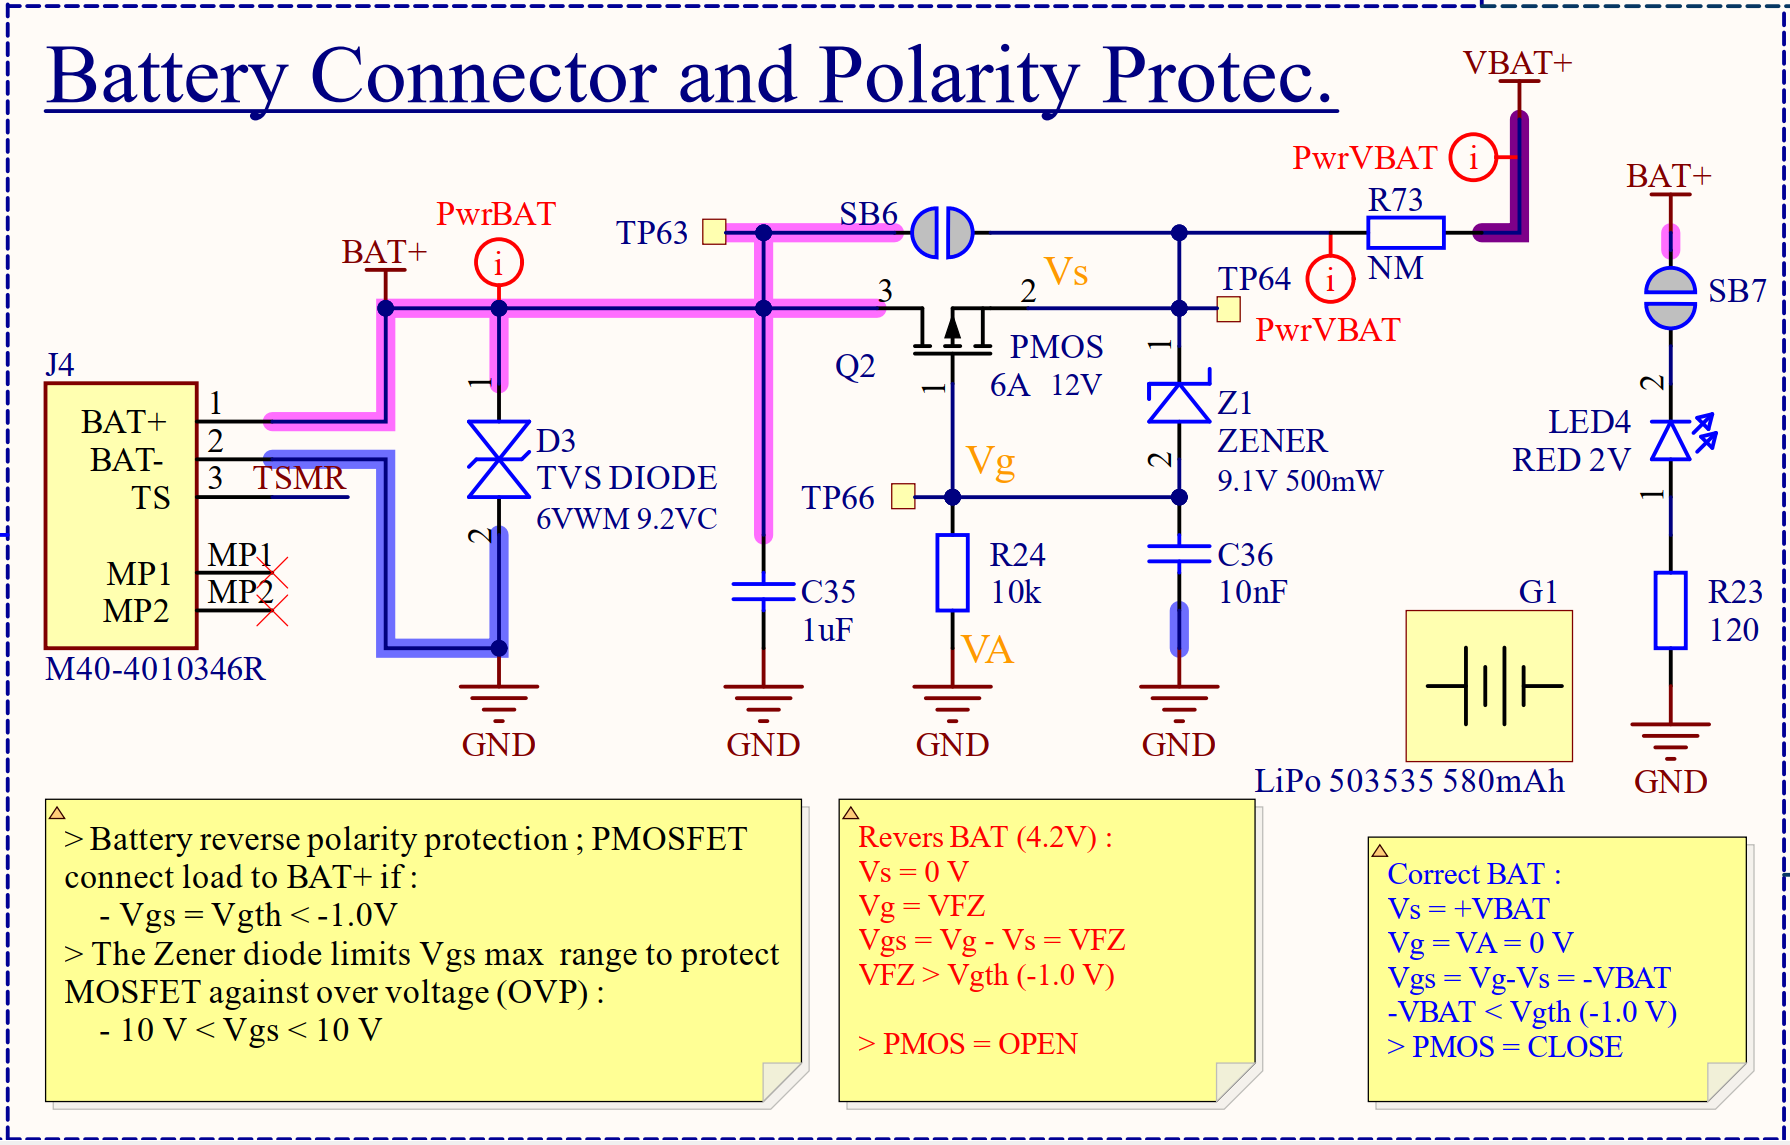
\includegraphics[width=0.9\textwidth]{Include/Figure/Hardware/LTEWatch_Power_Supply_Batt_Conn_Polarity_Protection}
	\caption{Power Supply : Battery Connector and Polarity Protection}
	\label{fig:LTEWatch_Power_Supply_Batt_Conn_Polarity_Protection}
\end{figure}

As the device is powered by battery, there is a risk of connecting the cell in reverse polarity which could seriously damage the circuit and in the worst case the battery if the reverse polarity connection results in a short circuit. The battery is connected with a 3-pin connector with a \textit{TS} line for battery thermal regulation.\\

The reverse polarity protection is achieved with a \textit{P-Chanel} MOSFET that act as a low loss reverse battery protection diode:
\begin{itemize}
\item $VBat > 0$ : $V_{gs} < V_{gth} \; \rightarrow$ PMOS is \textbf{\textcolor{mygreen}{ON}}
\item $VBat < 0$ : $V_{gs} > V_{gth} \; \rightarrow$ PMOS is \textbf{\textcolor{red}{OFF}}
\end{itemize}

The zener diode is used to limit the voltage range on the PMOS. The TVS diode is implemented for ESD protection. For direct revers battery indication, a red LED can be connected to +VBAT.\\

The \textit{P-Channel} MOSFET is the \textit{SSM3J332R}\cite{SSM3J332R} from \textsc{Toshiba}, which has the following specification:
\begin{itemize}
\item Gate threshold voltage : $V_{gth}= \SI{-1.2}{\volt}$ (max)
\item Drain–source on resistance : $R_{DS(ON)} = \SI{50}{\milli\ohm}$ ($V_{GS} = \SI{4.5}{\volt}$)
\item Gate-Source voltage range : $V_{GSS} = \pm \SI{12}{\volt}$
\item Drain current max : $I_D = \SI{-6}{\ampere}$
\item Power dissipation : $P_D = \SI{1}{\watt}$
\end{itemize}

\subsubsection{Battery Level Monitoring}

Battery level monitoring is mandatory in portable and wearable application. The simple battery level monitoring circuit of \textit{LTEWatch} is illustrated in figure \ref{fig:LTEWatch_Power_Supply_Batt_LVL_Monitoring}:

\begin{figure}[H]
	\centering
	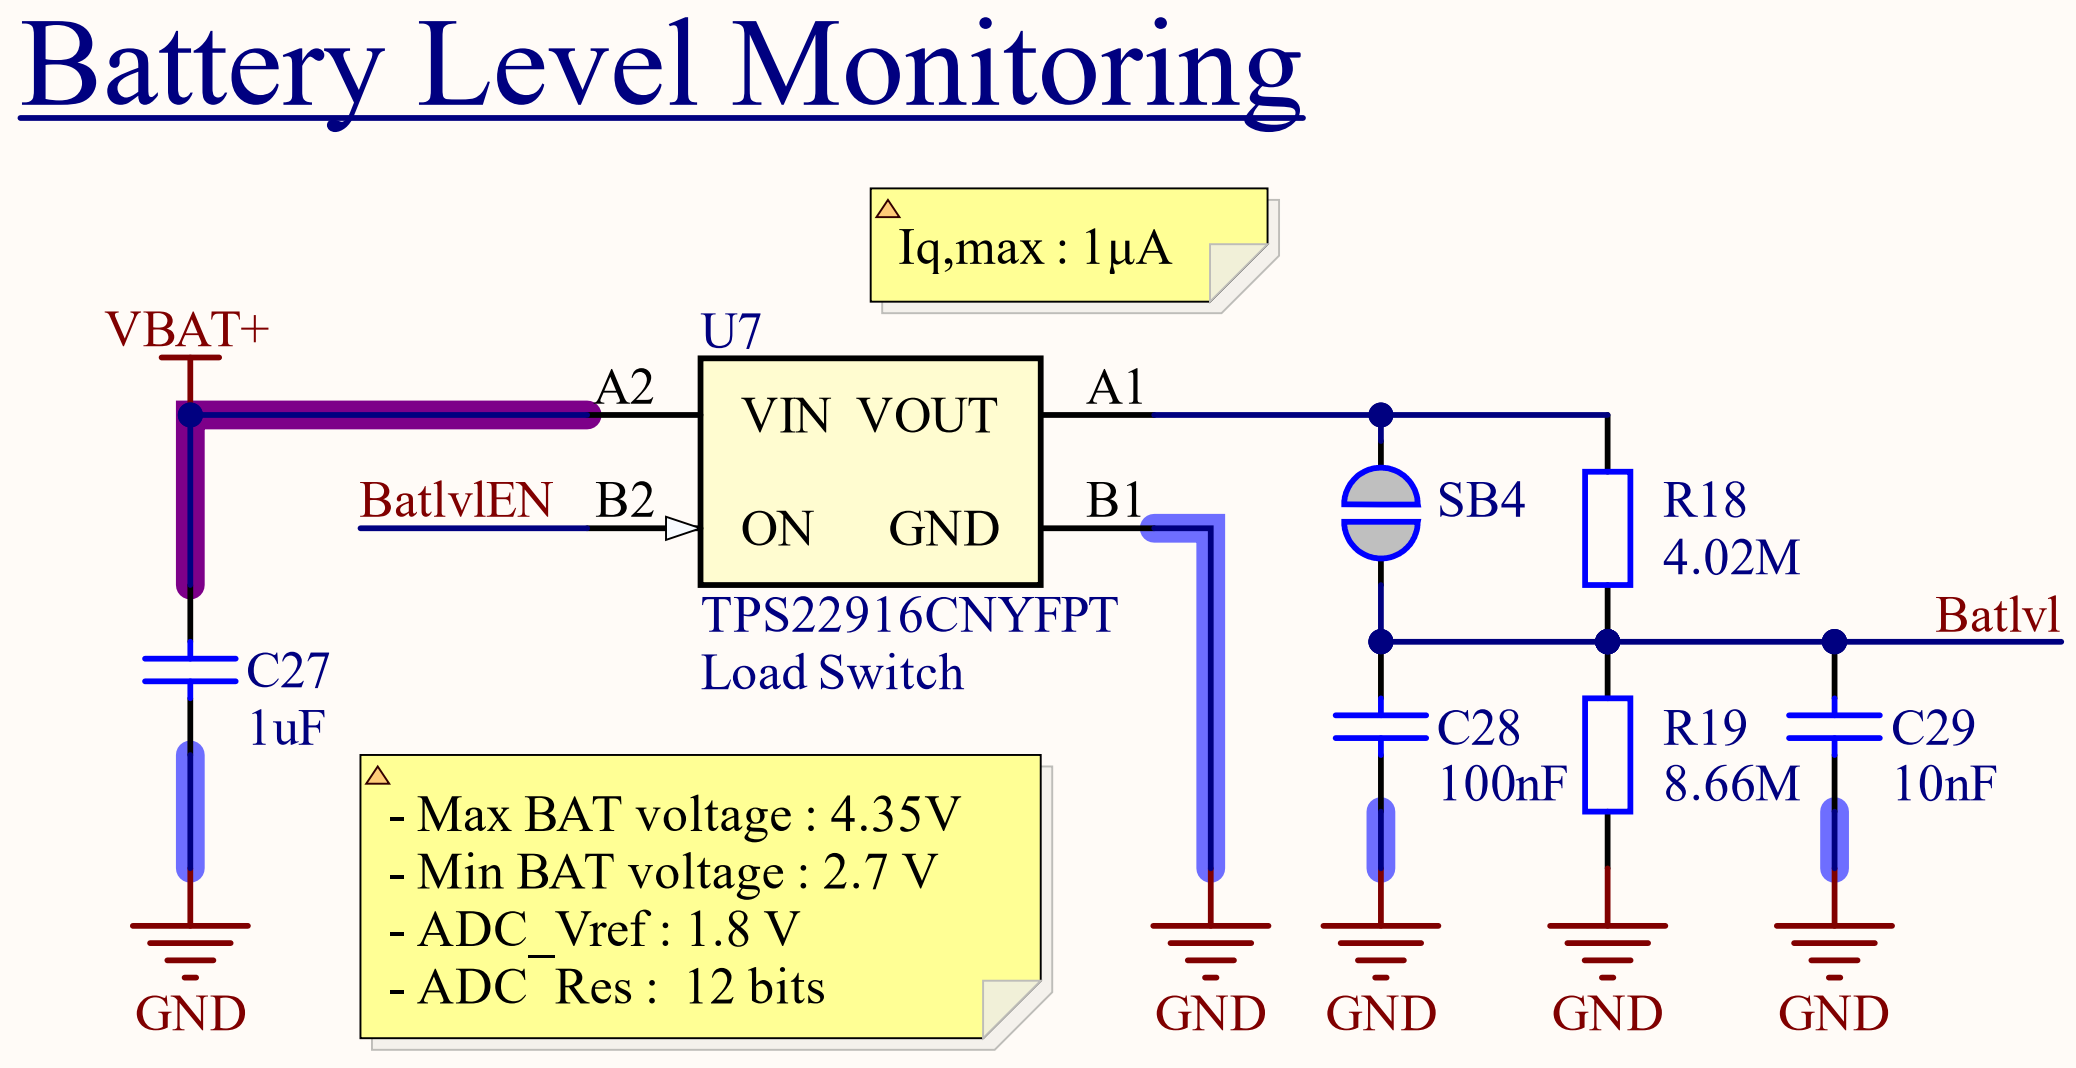
\includegraphics[width=0.8\textwidth]{Include/Figure/Hardware/LTEWatch_Power_Supply_Batt_LVL_Monitoring}
	\caption{Power Supply : Battery Level Monitoring}
	\label{fig:LTEWatch_Power_Supply_Batt_LVL_Monitoring}
\end{figure}

Battery level monitoring is directly measured by an ADC input of the \textit{nRF9160}. The measured battery voltage is adapted to the ADC range with a simple restive voltage divider:
$$
V_{meas} = V_{BAT} \cdot \dfrac{R_{19}}{R_{18} + R_{19}} = \ddl{0.683\cdot V_{BAT}}
$$
For a battery with $V_{BAT,FULL} = \SI{4.2}{\volt}$ and $V_{BAT,EMPTY} = \SI{3.0}{\volt}$:
\begin{itemize}
\item $V_{ADC,MAX} = \SI{2.868}{\volt}$ with $I_{BATLVL,MAX} = \SI{331}{\nano\ampere}$
\item $V_{ADC,MIN} = \SI{2.049}{\volt}$ with $I_{BATLVL,MIN} = \SI{237}{\nano\ampere}$
\end{itemize}

In order to reduce current consumption, a load switch is added to enable or disable the battery level monitoring. The load switch typical current consumption is:
\begin{itemize}
\item \textbf{\textcolor{mygreen}{ON}} state: $I_{BATLVL,MAX} =  \SI{500}{\nano\ampere} > I_{BATLVL,MIN}$
\item \textbf{\textcolor{red}{OFF}} state: $I_{BATLVL,MIN} = \SI{10}{\nano\ampere} < I_{BATLVL,MIN}$
\end{itemize} 
This means that current consumption is reduced if:
$$
\begin{array}{c}
\bigg(\overbrace{\dfrac{t_h}{t_h+t_l}}^{D}\bigg) \cdot \SI{500}{\nano\ampere} + \bigg(\overbrace{\dfrac{t_l}{t_h+t_l}}^{1-D}\bigg) \cdot \SI{10}{\nano\ampere} < \SI{237}{\nano\ampere}\\[15pt]
	\rightarrow D \cdot \SI{500}{\nano\ampere} + (1-D)\cdot \SI{10}{\nano\ampere} < \SI{237}{\nano\ampere}\\[12pt]
\rightarrow \quad D \cdot \SI{490}{\nano\ampere} < \SI{237}{\nano\ampere} \Rightarrow \quad \ddl{D < \SI{48}{\percent}}
\end{array}
$$

The load switch effectively reduces the current consumption of battery level monitoring, as long as \textbf{\textcolor{mygreen}{ON}} state duty cycle is less than \SI{48}{\percent}.

\subsubsection{Li-Ion Battery Charger and Protection Unit}

The battery charger and protection unite implement the \textit{BQ25180} from \textsc{Texas Instrument}. The electrical schematic of the battery charger unit is illustrated in figure \ref{fig:LTEWatch_Power_Supply_Li_Ion_Batt}:
\begin{figure}[H]
	\centering
	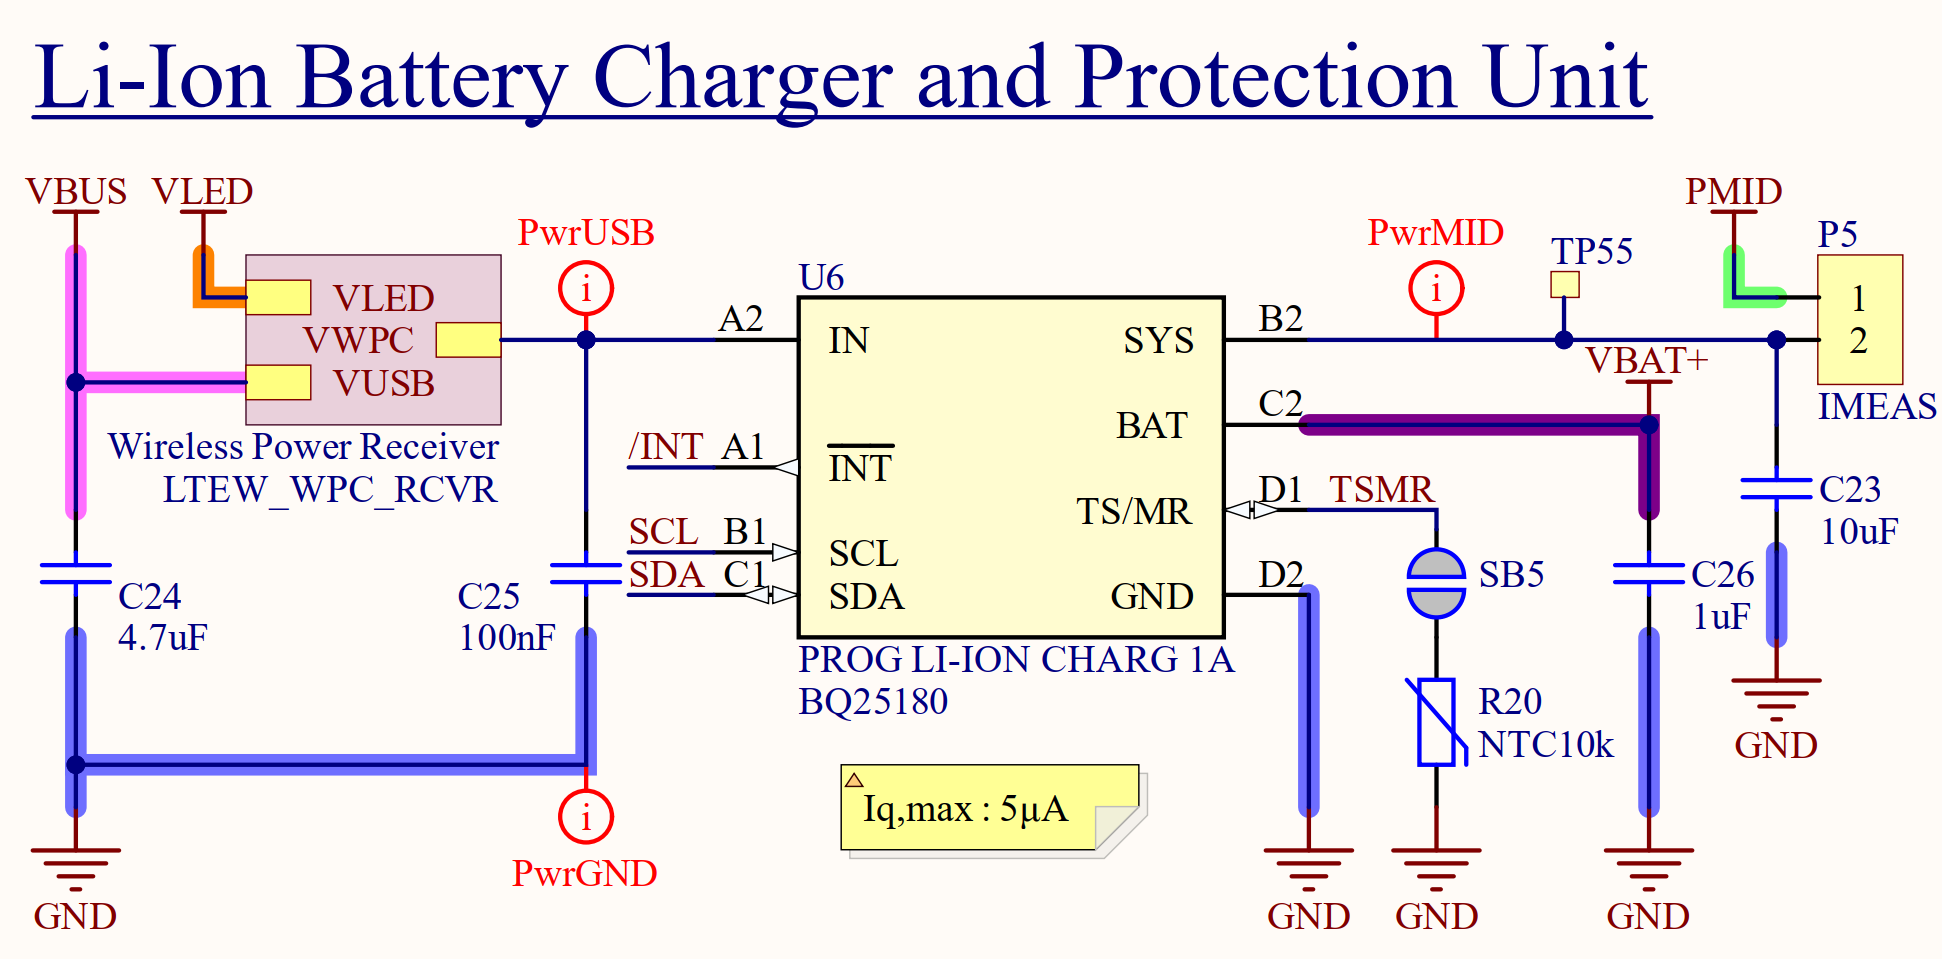
\includegraphics[width=0.85\textwidth]{Include/Figure/Hardware/LTEWatch_Power_Supply_Li-Ion_Batt}
	\caption{Power Supply : Li-Ion Battery Charger and Protection Unit}
	\label{fig:LTEWatch_Power_Supply_Li_Ion_Batt}
\end{figure}

The integration of the \textit{BQ25180} is very straightforward, the values of capacitors $C_{23}$, $C_{24}$, $C_{25}$ and $C_{26}$ have been chosen following the design recommendation describes on page \pageref{sec:bat_chrg_sel}. This unit also contains a \SI{10}{\kilo\ohm} \textit{NTC} that can be connected to the \textit{BQ25180} with a solder bridge and \textit{"IMEAS"} jumper that can be unplug to measure the current consumption of the system.

\subsubsection{+3V3 Buck-Boost Converter}

Figure \ref{fig:LTEWatch_Power_Supply_3V3_Buck_Boost} illustrates the electrical schematic of the \textit{+3V3 Buck-Boost} unit:

\begin{figure}[H]
	\centering
	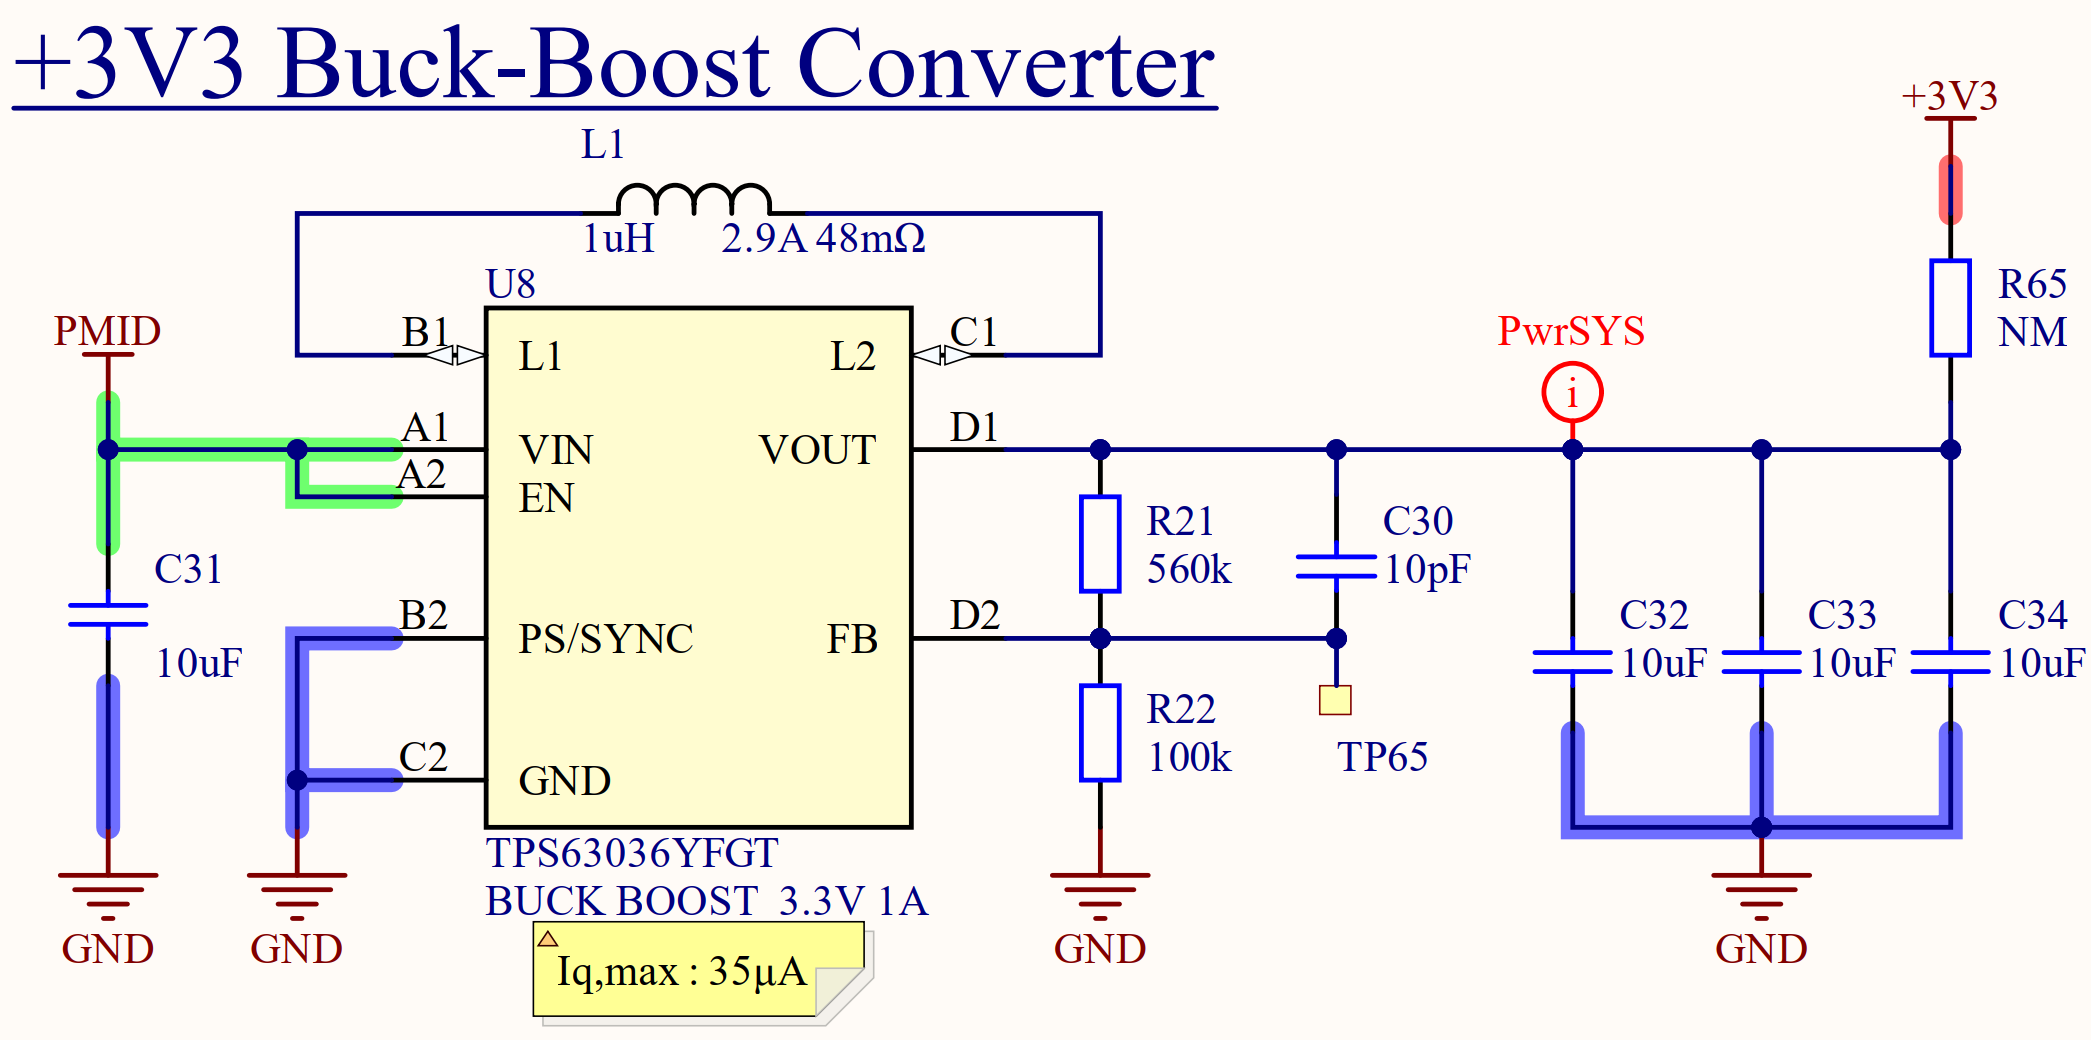
\includegraphics[width=1\textwidth]{Include/Figure/Hardware/LTEWatch_Power_Supply_3V3_Buck-Boost}
	\caption{Power Supply : $+3V3$ Buck-Boost Converter}
	\label{fig:LTEWatch_Power_Supply_3V3_Buck_Boost}
\end{figure}

The most critical components of the circuit illustrated in figure \ref{fig:LTEWatch_Power_Supply_3V3_Buck_Boost} are the inductor $L_1$ and the voltage divider resistances $R_{21}$ and $R_{22}$. Their value were determined using the design recommendation of the \textit{TPS63036} describes on page \pageref{sec:bck_bst_sel}.

\subsubsection{+1V8 GPIO LDO}

Figure \ref{fig:LTEWatch_Power_Supply_1V8_GPIO} illustrates the electrical schematic of the \textit{+1V8 GPIO LDO} unit:

\begin{figure}[H]
	\centering
	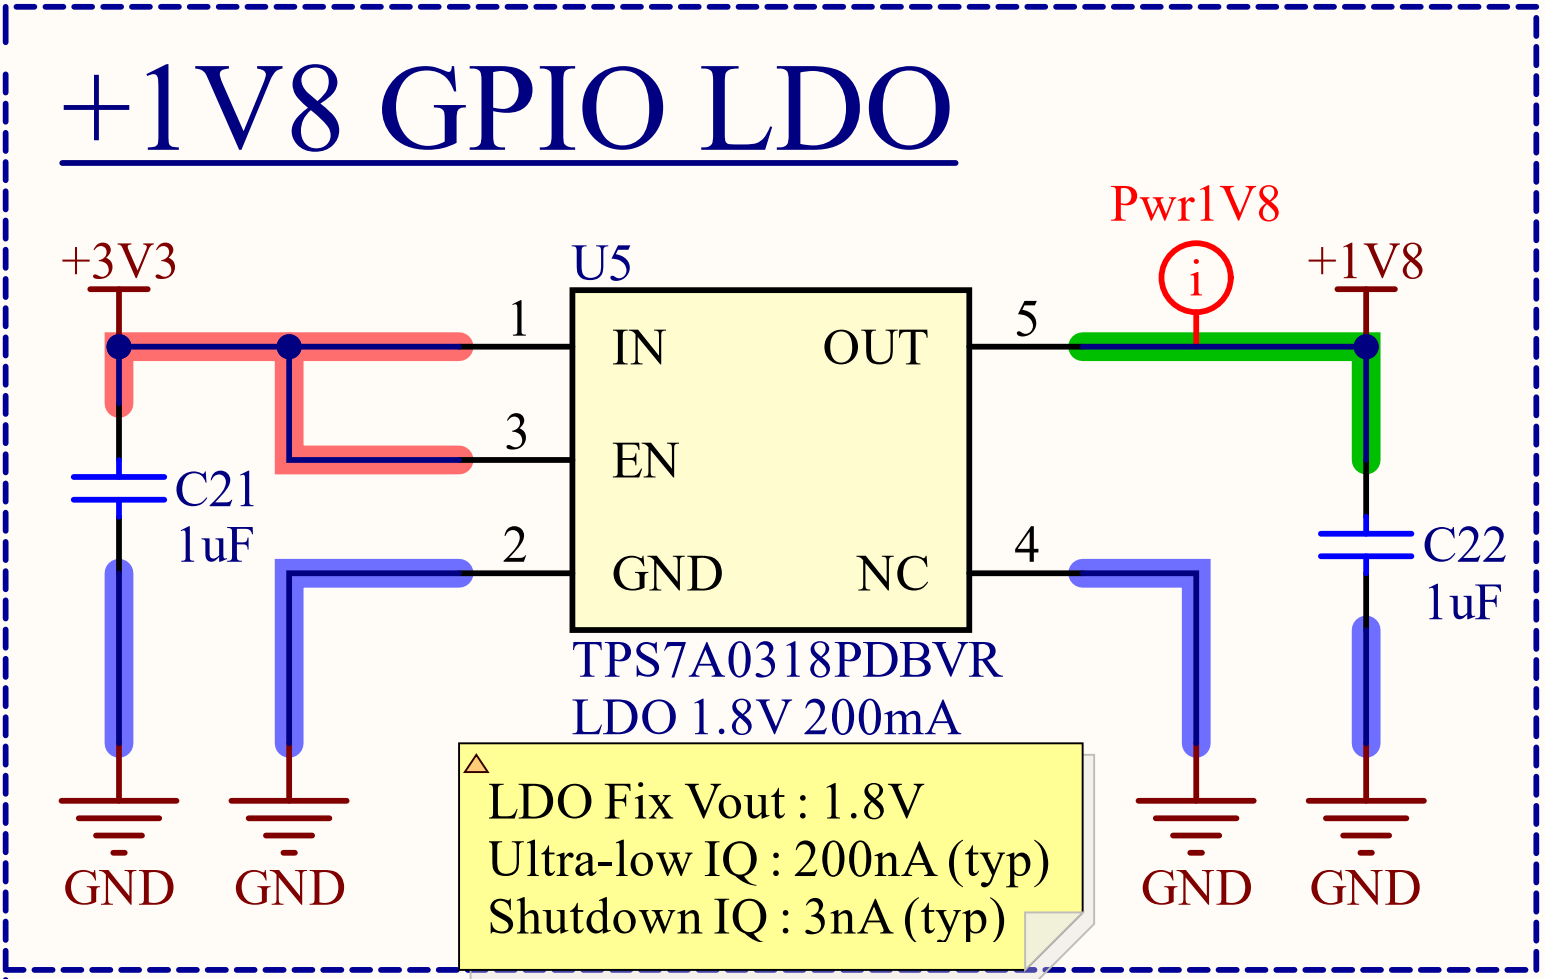
\includegraphics[width=0.65\textwidth]{Include/Figure/Hardware/LTEWatch_Power_Supply_1V8_GPIO}
	\caption{Power Supply : $+1V8$ GPIO LDO}
	\label{fig:LTEWatch_Power_Supply_1V8_GPIO}
\end{figure}

This circuit only integrates the \textit{TPS7A03} \SI{1.8}{\volt} \textit{LDO} regulator. We can see that the schematic of the figure \ref{fig:LTEWatch_Power_Supply_1V8_GPIO} is very simple. The only external component required are the coupling capacitors $C_{21}$ and $C_{22}$. Their values correspond to those of the design recommendation described on page \pageref{sec:ldo_reg_sel}.

\subsubsection{Wireless Power Receiver (WPC/QI)}

The \textit{Wireless Power Receiver (WPC/QI)} unit integrates the \textit{BQ51013B} from \textsc{Texas Instrument}. The schematic of this unit is shown in figures \ref{fig:LTEWatch_WPC_RCVR_WPC} to \ref{fig:LTEWatch_WPC_RCVR_WPC_Enable}:

\begin{figure}[H]
	\centering
	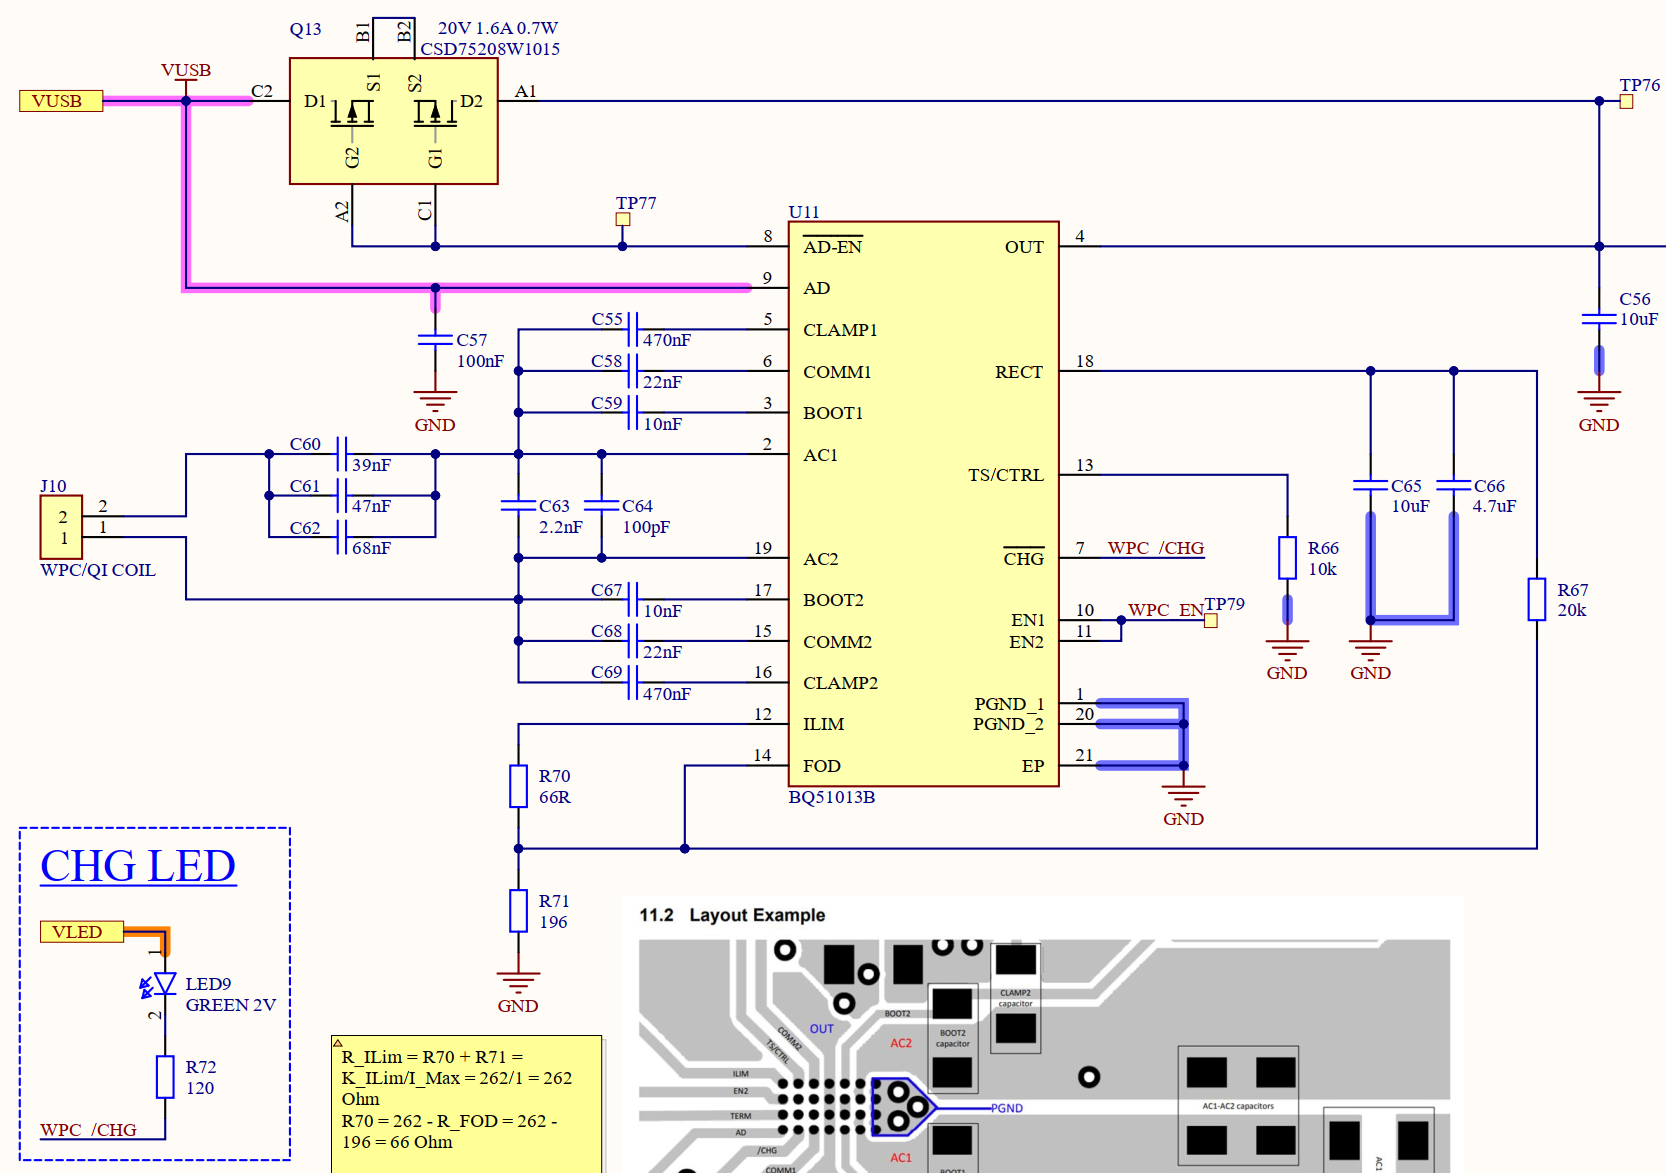
\includegraphics[width=1\textwidth]{Include/Figure/Hardware/LTEWatch_WPC_RCVR_WPC}
	\caption{Power Supply : Wireless Power Receiver (WPC/QI)}
	\label{fig:LTEWatch_WPC_RCVR_WPC}
\end{figure}

Figure \ref{fig:LTEWatch_WPC_RCVR_WPC} illustrates the electrical schematic of the \textit{BQ51013B}.\\


The integration of the (\textit{WPC/QI}) power receiver is less trivial than units previously described. The schematic is decomposed in the following blocks:
\begin{enumerate}
\item Power Receiver (\textit{WPC/QI}) chip (\textit{BQ51013B})
\item Power supply blocking \textit{FET} (\textit{CSD75208W1015})
\item Charging state indicator (\textit{LED9})
\item Power Receiver (\textit{WPC/QI}) enable circuit ($R_{68}$, $R_{69}$ and $Q_{14}$)\\
\end{enumerate}

The integration process of the \textit{BQ51013B} is describes in detail in the design recommendation of the component on page \pageref{sec:wpc_rcvr_sel}. The most critical part of the implementation of the \textit{BQ51013B} is the the determination of receiver coil dual resonant circuit series capacitors $C_{60}$, $C_{61}$, $C_{62}$, and parallel capacitors $C_{63}$ and $C_{64}$. The guideline to calculate those component is also described on page \pageref{sec:wpc_rcvr_sel}.\\

\pagebreak

The second block is the power supply block \textit{FET} (\textit{CSD75208W1015}), this component is a \textit{P-Channel} \textit{FET} pair. When the \textit{USB} bus is supplied ($V_{BUS} = \SI{+5}{\volt}$), the pin \textit{AD} is set 'high' and the pin $\overline{\text{AD-EN}}$ is set to 'low'. In this state, the blocking \textit{FET} lets pass the power supply from VUSB. Conversely, when VBUS is not supplied ($V_{BUS} = \SI{0}{\volt}$) the blocking \textit{FET} disconnect VBUS line from the load system. \\

The third block is the charging state indicator, which is simply a LED in series with a resistance to limit current. The calculation of the value of $R_{72}$ is described in the design recommendations on page \pageref{sec:wpc_rcvr_sel}.\\

The last block is the \textit{WPC} enable control circuit, which is simply an inverting \textit{N-Channel}  MOSFET switch. The schematic of this block is illustrated in figure \ref{fig:LTEWatch_WPC_RCVR_WPC_Enable}:

\begin{figure}[H]
	\centering
	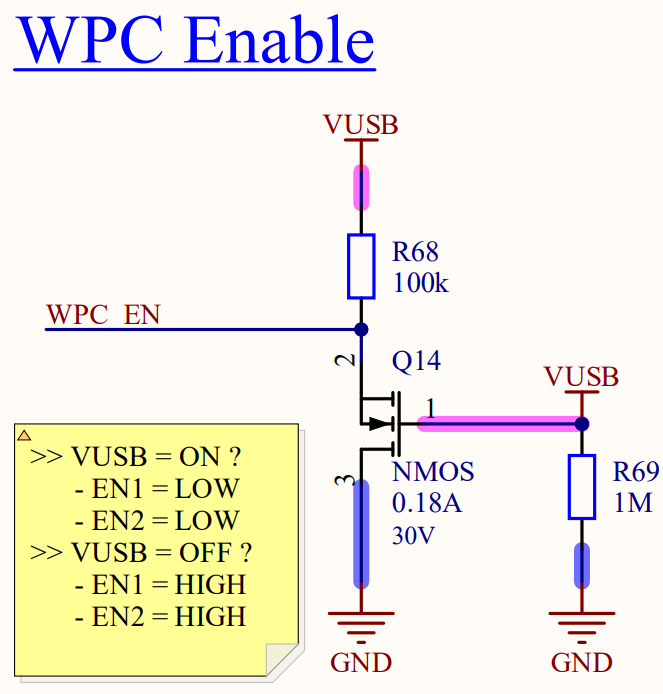
\includegraphics[width=0.5\textwidth]{Include/Figure/Hardware/LTEWatch_WPC_RCVR_WPC_Enable}
	\caption{Power Supply : Wireless Power Receiver (WPC/QI) Enable}
	\label{fig:LTEWatch_WPC_RCVR_WPC_Enable}
\end{figure}

% ------------------------------ MCU -------------------------------------

\subsection{MCU System (\textit{nRF9160})}

The \textit{MCU} System block contains all units relative to the \textit{nRF9160}, which are decomposed as follow:
\begin{enumerate}
\item \textit{nRF9160} SiP
\item FTDI-UART \textit{USB-to-UART} interface
\item USB-C and JTAG connectors
\item GPS EXTINT : +1V8 MAGPIO to +3V3 GNSS EXT INT level shifter
\item SIM and eSIM connectors
\end{enumerate}

\pagebreak

\subsubsection{nRF9160 SiP}

The electrical schematic of the \textit{nRF9160} SiP is illustrated in figure \ref{fig:LTEWatch_nRF9160_nRF9160}:

\begin{figure}[H]
	\centering
	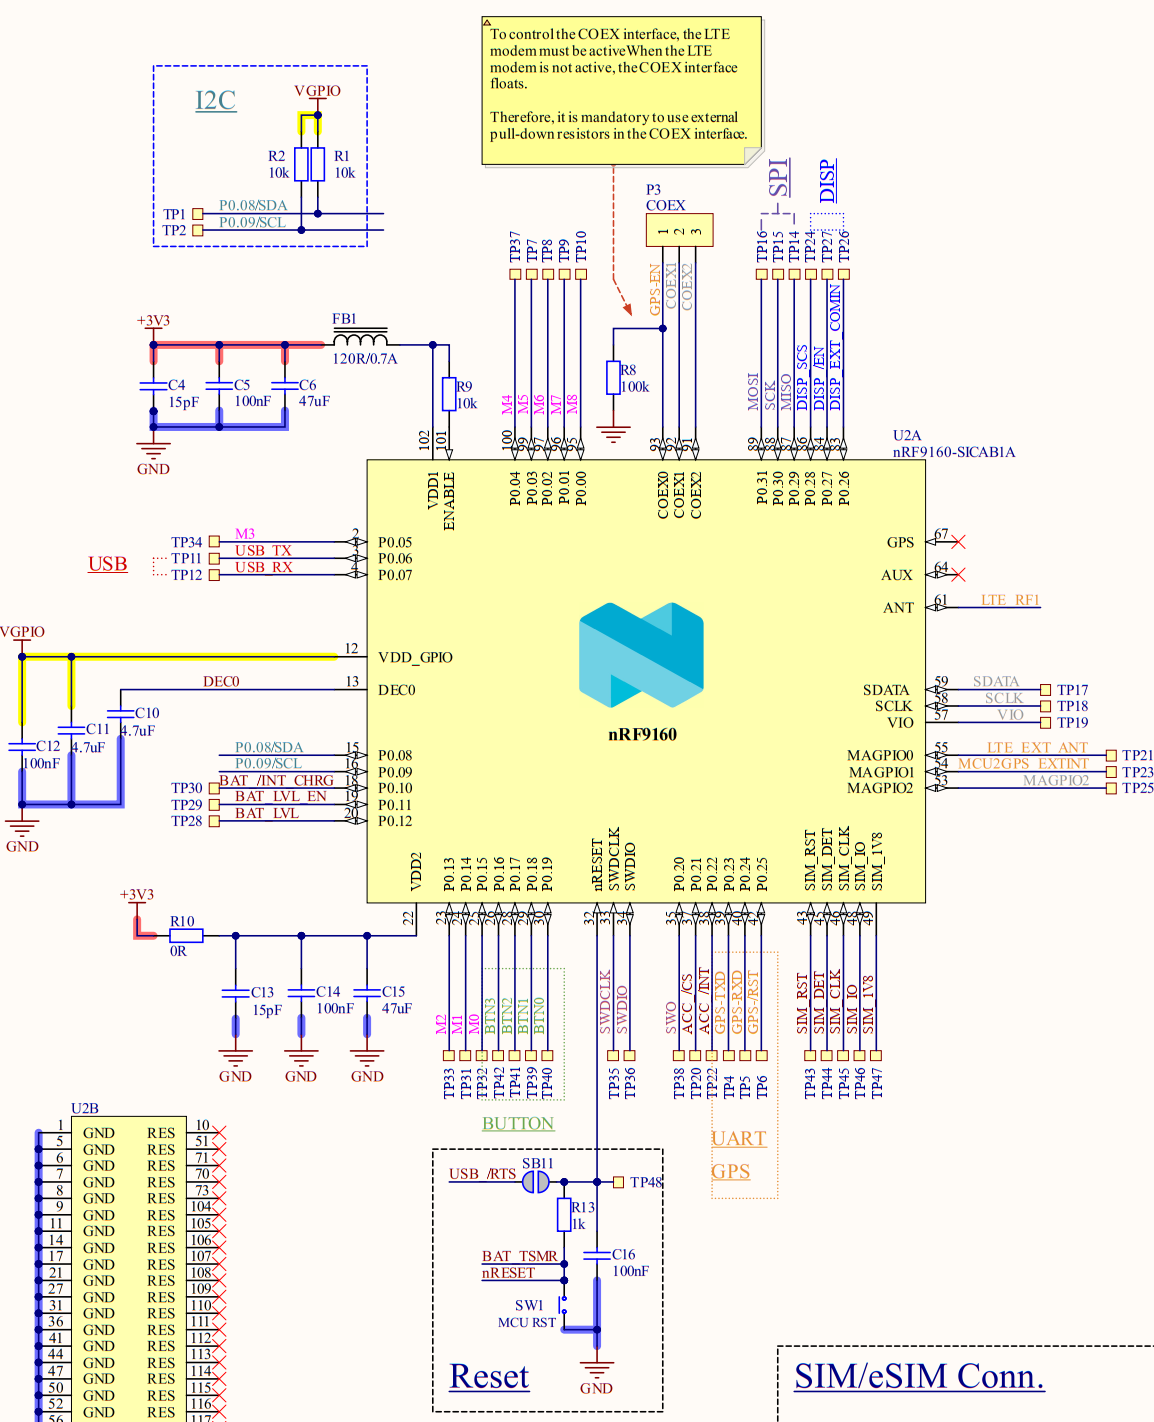
\includegraphics[width=1\textwidth, angle=0]{Include/Figure/Hardware/LTEWatch_nRF9160_nRF9160}
	\caption{nRF9160 : nRF9160}
	\label{fig:LTEWatch_nRF9160_nRF9160}
\end{figure}

\pagebreak

The integration shown in figure \ref{fig:LTEWatch_nRF9160_nRF9160} is based on the board schematic of the \textit{nRF9160DK}\cite{nRF9160DK}, the pin assignment varies, but the values of external components are identical. A noticeable difference is the \textit{nRESET} pin which is connected to a push button like the \textit{nRF9160DK} board, but is also connected to the battery charger \textit{TSMR} pin which is also used as a /RESET pin. \\

We can see from the schematic that the \textit{MCU} is well populated and almost all the pins are used. Even COEX0 is used as \textit{GPS-EN} output, MAGPIO0 and MAGPIO1 are used, respectively for external LTE antenna configuration (\textit{LTE\_EXT\_ANT}) and as GNSS interrupt output (\textit{MCU2GPS\_EXTINT}).\\

The reason the \textit{MCU} is cluttered is that I'm adding lots of options and extra configuration to keep the prototype board versatile and to keep back-up plans in case of mistakes while designing the board or unfortunate discoveries during the software development.

\subsubsection{FTDI - UART}

Figure \ref{fig:LTEWatch_nRF9160_FTDI_UART} illustrates the electrical schematic of the FTDI-UART \textit{USB-to-UART} interface circuit:

\begin{figure}[H]
	\centering
	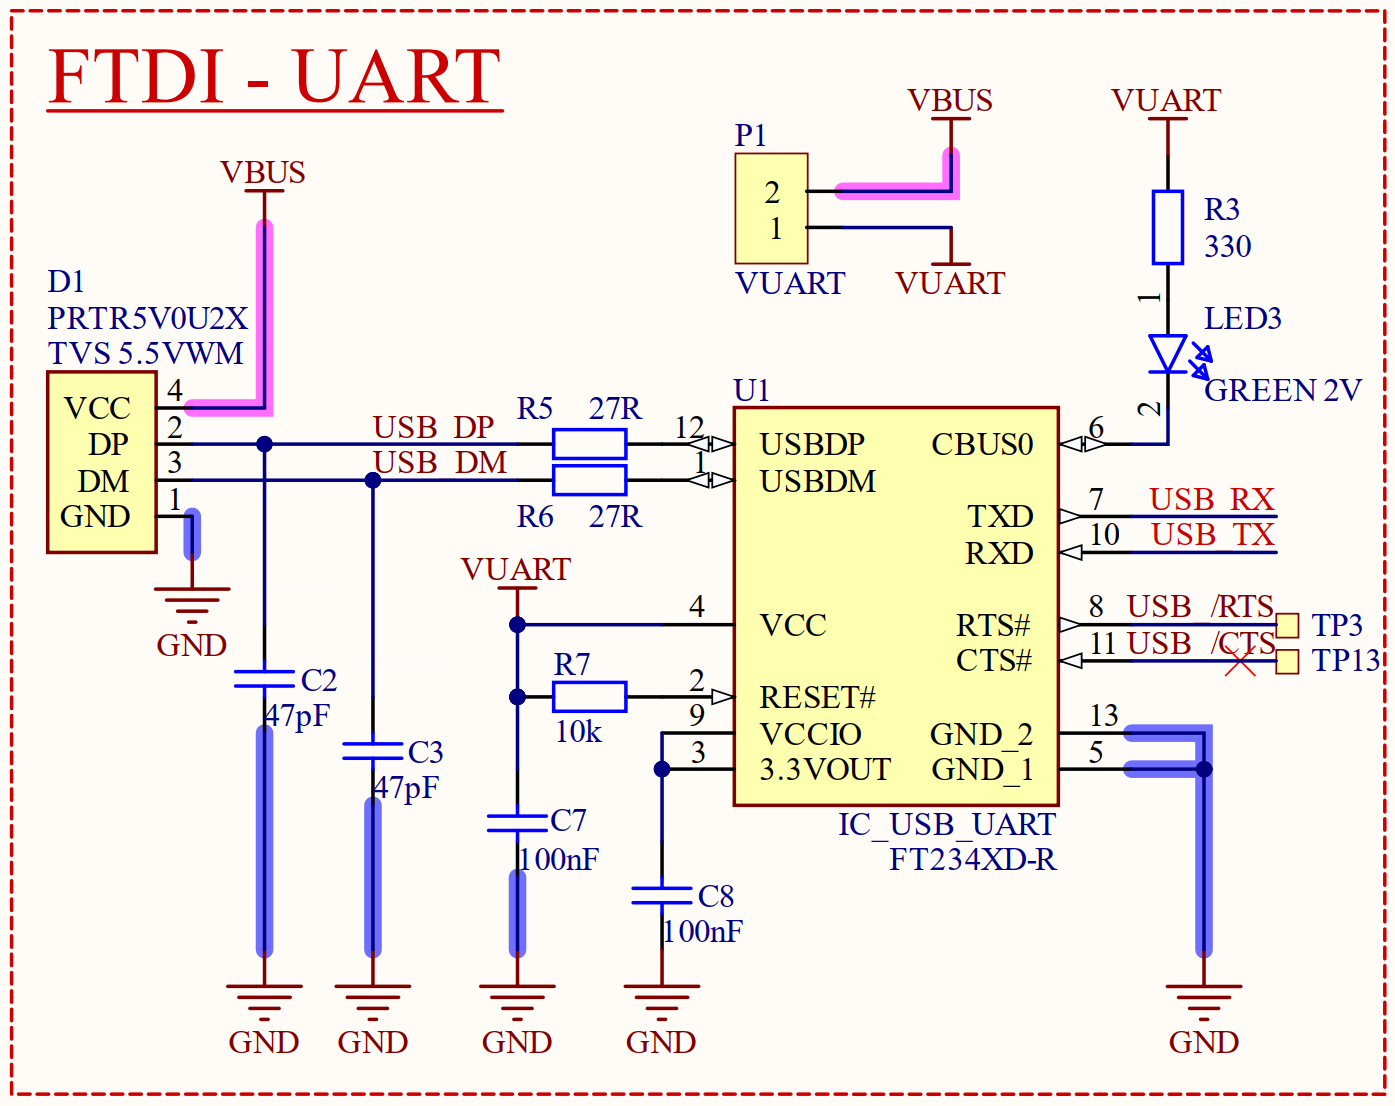
\includegraphics[width=0.8\textwidth]{Include/Figure/Hardware/LTEWatch_nRF9160_FTDI-UART}
	\caption{nRF9160 : FTDI-UART}
	\label{fig:LTEWatch_nRF9160_FTDI_UART}
\end{figure}

As shown in figure \ref{fig:LTEWatch_nRF9160_FTDI_UART}, the FTDI-UART interface module is the \textit{FT234XD-R}. This implementation is based on the \textit{typical USB bus power configuration} described on page \pageref{sec:ftdi_usb_app}.\\

Due to the limited number of pins still available on the \textit{nRF9160}, the \textit{RTS} and \textit{CTS} signals are not connected to the \textit{MCU} and therefore not used. The \textit{FT234XD-R} can drive a \textit{TX/RX} LED indicator on the pin CBUS0. This pin is internally pulled-down.\\

The component on the left (D1), which is a (\textit{PRTR5V0U2X}\cite{PRTR5V0U2X}), is an ultra low capacitance double rail-to-rail \textit{ESD} protection diode suitable for USB bus.\\

Concerning the external passive components, the datasheet of the \textit{FT234XD-R}\cite{FTDIUSB} recommended adding small \SI{25}{\ohm} series resistors to the USB bus to limit current. It was also recommended to add a ferrite bead on the VUSB power supply line to reduce \textit{EMI} noise from the \textit{FT234XD} and associated circuitry being radiated down the USB cable to the USB host. The ferrit bead is present on the \textit{USB-C/JTAG} block (fig.\ref{fig:LTEWatch_nRF9160_USBC_JTAG}). More details are described in the design recommendations of the component on page \pageref{sec:ftdi_sel}.

\subsubsection{GPS EXTINT}

Figure \ref{fig:LTEWatch_nRF9160_GPS_EXTINT} illustrates the electrical schematic of the \textit{GPS EXTINT} block:

\begin{figure}[H]
	\centering
	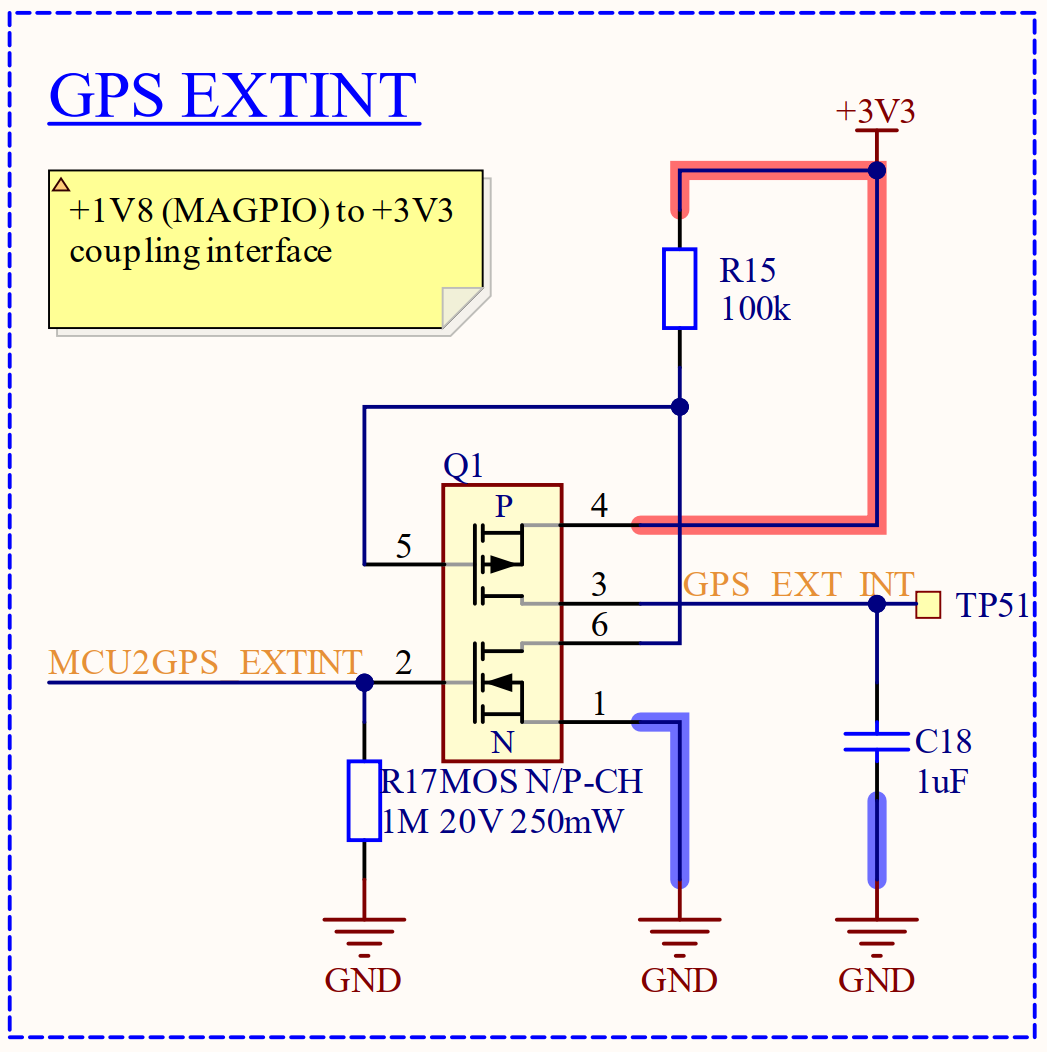
\includegraphics[width=0.55\textwidth]{Include/Figure/Hardware/LTEWatch_nRF9160_GPS_EXTINT}
	\caption{nRF9160 : GPS EXTINT}
	\label{fig:LTEWatch_nRF9160_GPS_EXTINT}
\end{figure}

The \textit{GNSS} receiver has an external interrupt (EXT\_INT) input that can be used by the \textit{MCU} to send interrupts to the \textit{GNSS} module. Due to the overcrowded \textit{GPIOs} of the \textit{nRF9160}, the only solution to add this signal was to connect it on one of the \textit{MAGPIO} pin of the \textit{nRF9160}. \textit{MAGPIO} is IO port of the modem that is integrated in the \textit{nRF9160}. The problem with this port is the only compatibility with $1.8V$ \textit{GPIO}. The \textit{GNSS} requiring at least \SI{2.7}{\volt} to detect a \textit{'high'}, it is necessary to interface this pin with a level shiffter for \SI{3.0}{\volt} designs. The level shifter is simply implemented with a non inverting dual MOSFET switch.

\subsubsection{USB-C / JTAG}

The \textit{USB-C/JTAG} block contains two connectors:
\begin{enumerate}
\item USB-C: This connector provides USB power supply and can also be interfaced with c custom JTAG to USB-C interface that can be developed later.
\item JTAG (SWIO): Standard connector for \textit{J-Link} programmer from \textsc{Segger} This connector can also be used directly with other \textit{nRF} development Kit from \textsc{Nordic Semi}.
\end{enumerate}

The electrical schematic of the textit{USB-C/JTAG} block is illustrated in the figure \ref{fig:LTEWatch_nRF9160_USBC_JTAG}:

\begin{figure}[H]
	\centering
	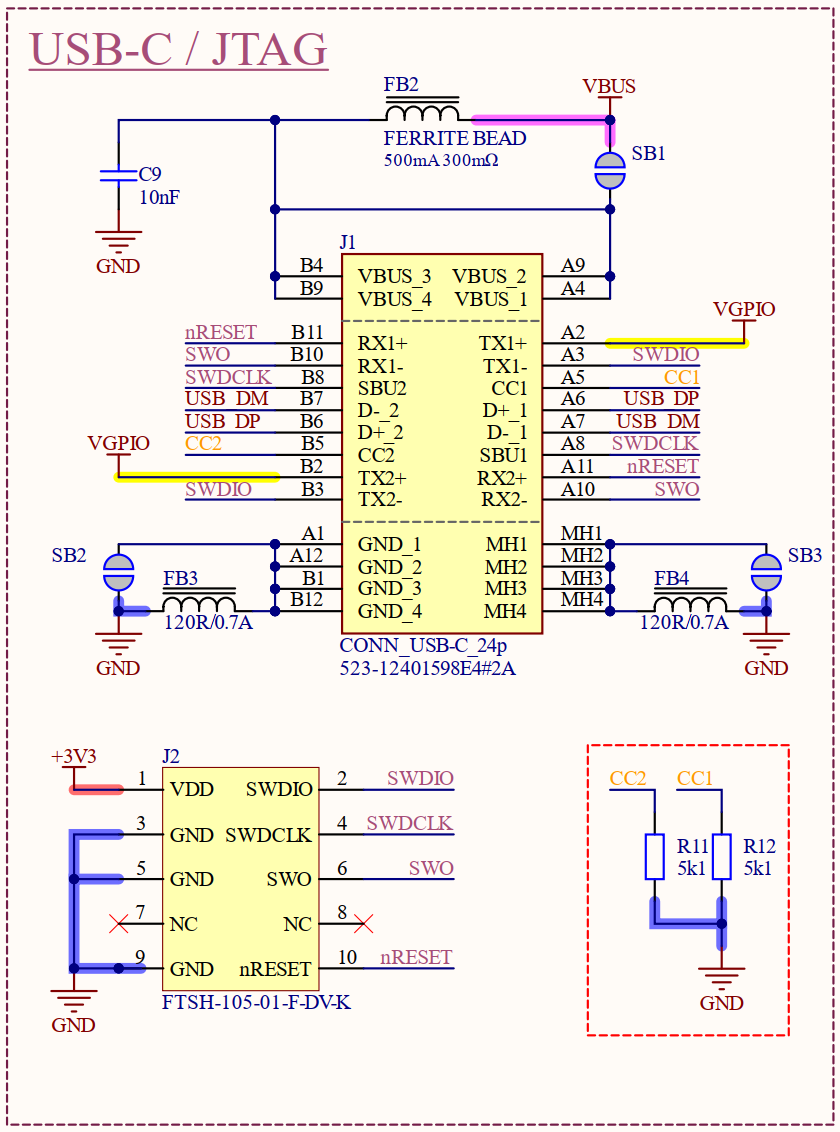
\includegraphics[width=0.75\textwidth]{Include/Figure/Hardware/LTEWatch_nRF9160_USB-C_JTAG}
	\caption{nRF9160 : USB-C / JTAG}
	\label{fig:LTEWatch_nRF9160_USBC_JTAG}
\end{figure}

As shown on figure \ref{fig:LTEWatch_nRF9160_USBC_JTAG}, the USB-C connector uses three ferrite bead filters that can be connected with solder bridge if needed. This filter are used to reduce \textit{EMI} noise from the USB-C host and cable.

\pagebreak
\subsubsection{SIM/eSIM Connector}

This block integrates connectors for both SIM and eSIM cards. The electrical schematic of this block is illustrated in figure \ref{fig:LTEWatch_nRF9160_SIM_eSIM}:

\begin{figure}[H]
	\centering
	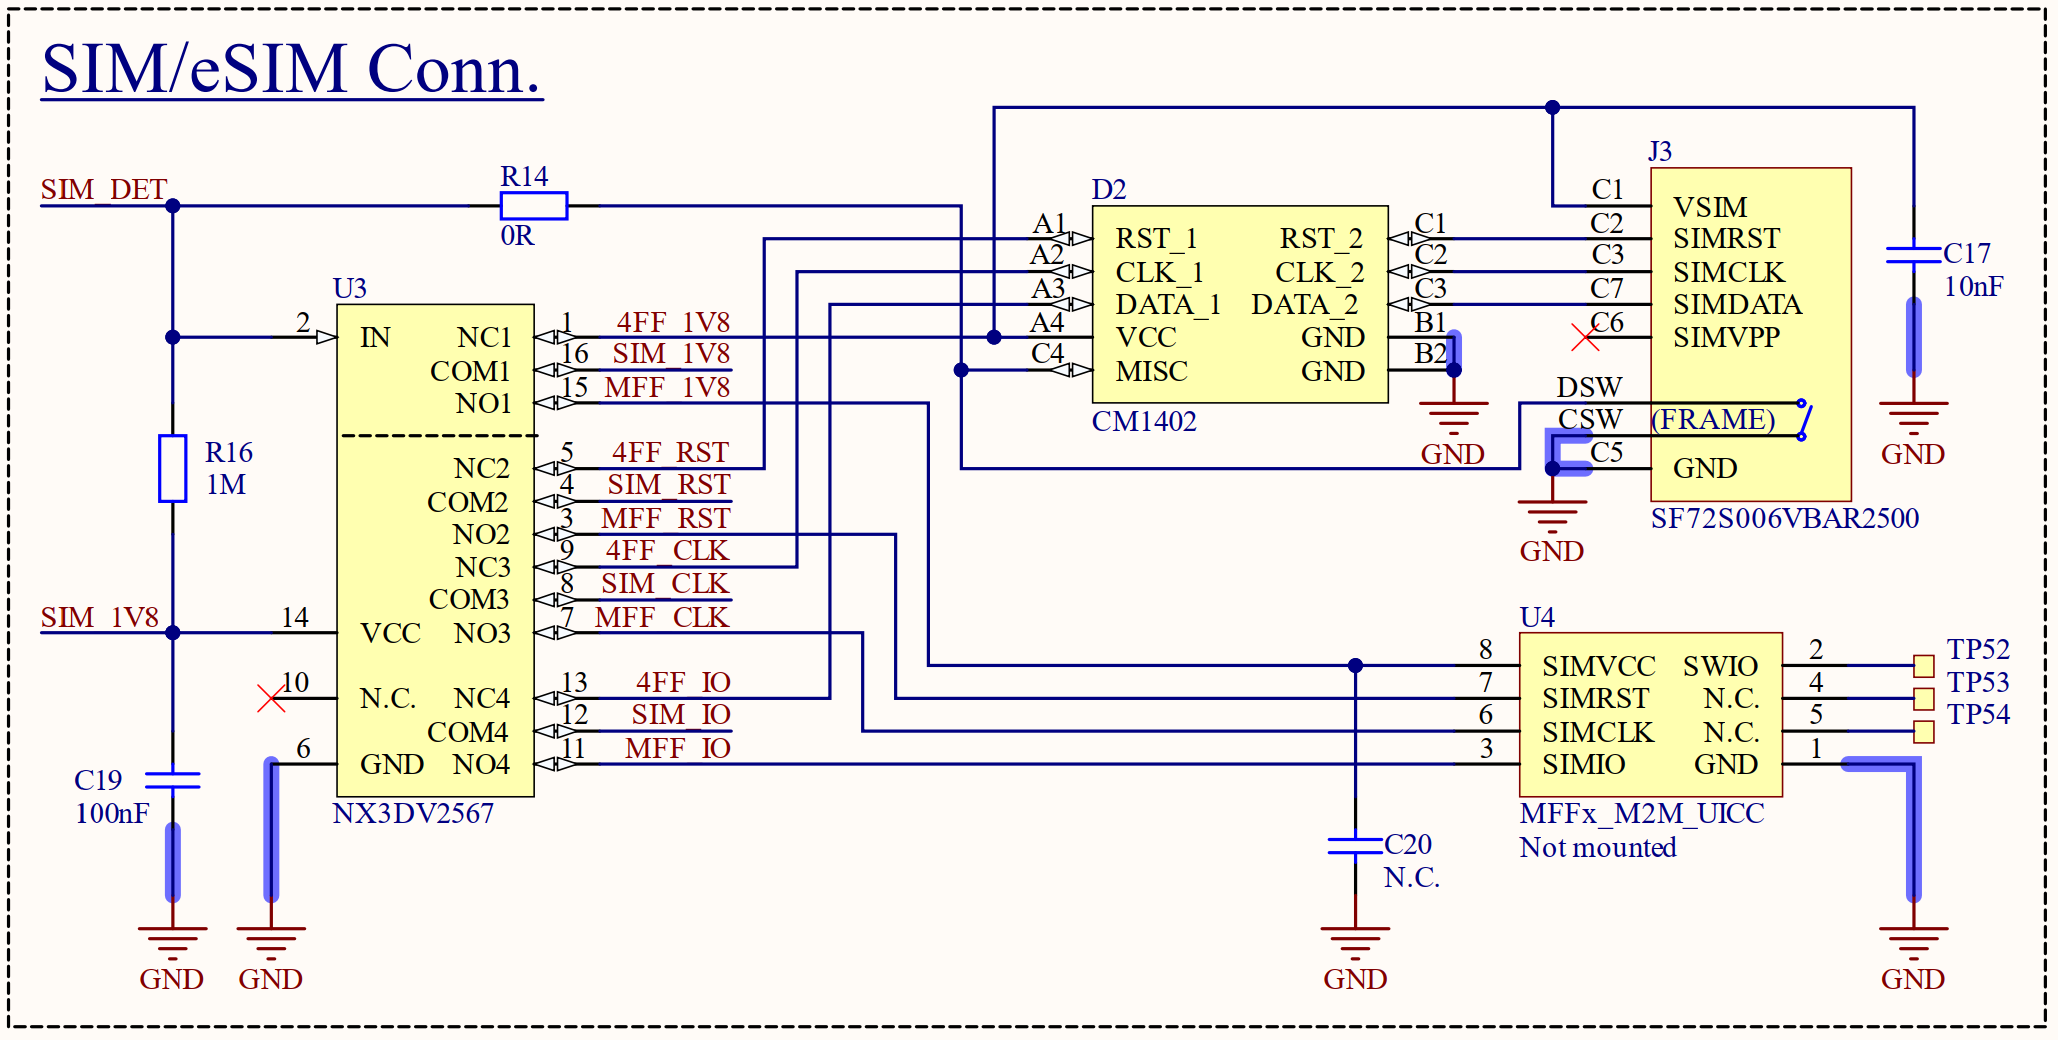
\includegraphics[width=1\textwidth]{Include/Figure/Hardware/LTEWatch_nRF9160_SIM_eSIM}
	\caption{nRF9160 : SIM/eSIM Connector}
	\label{fig:LTEWatch_nRF9160_SIM_eSIM}
\end{figure}

The schematic shown in figure \ref{fig:LTEWatch_nRF9160_SIM_eSIM} is based on the schematic from the \textit{thingy91}\cite{thingy91} board from \textsc{Nordic Semi.} This schematic also respects Sim card interface recommendations from the \textit{"Product Specification"}\cite{nRF9160} of the \textit{nRF9160}, which has the topology shown in figure \ref{fig:nrf9160_sim_interf}:

\begin{figure}[H]
	\centering
	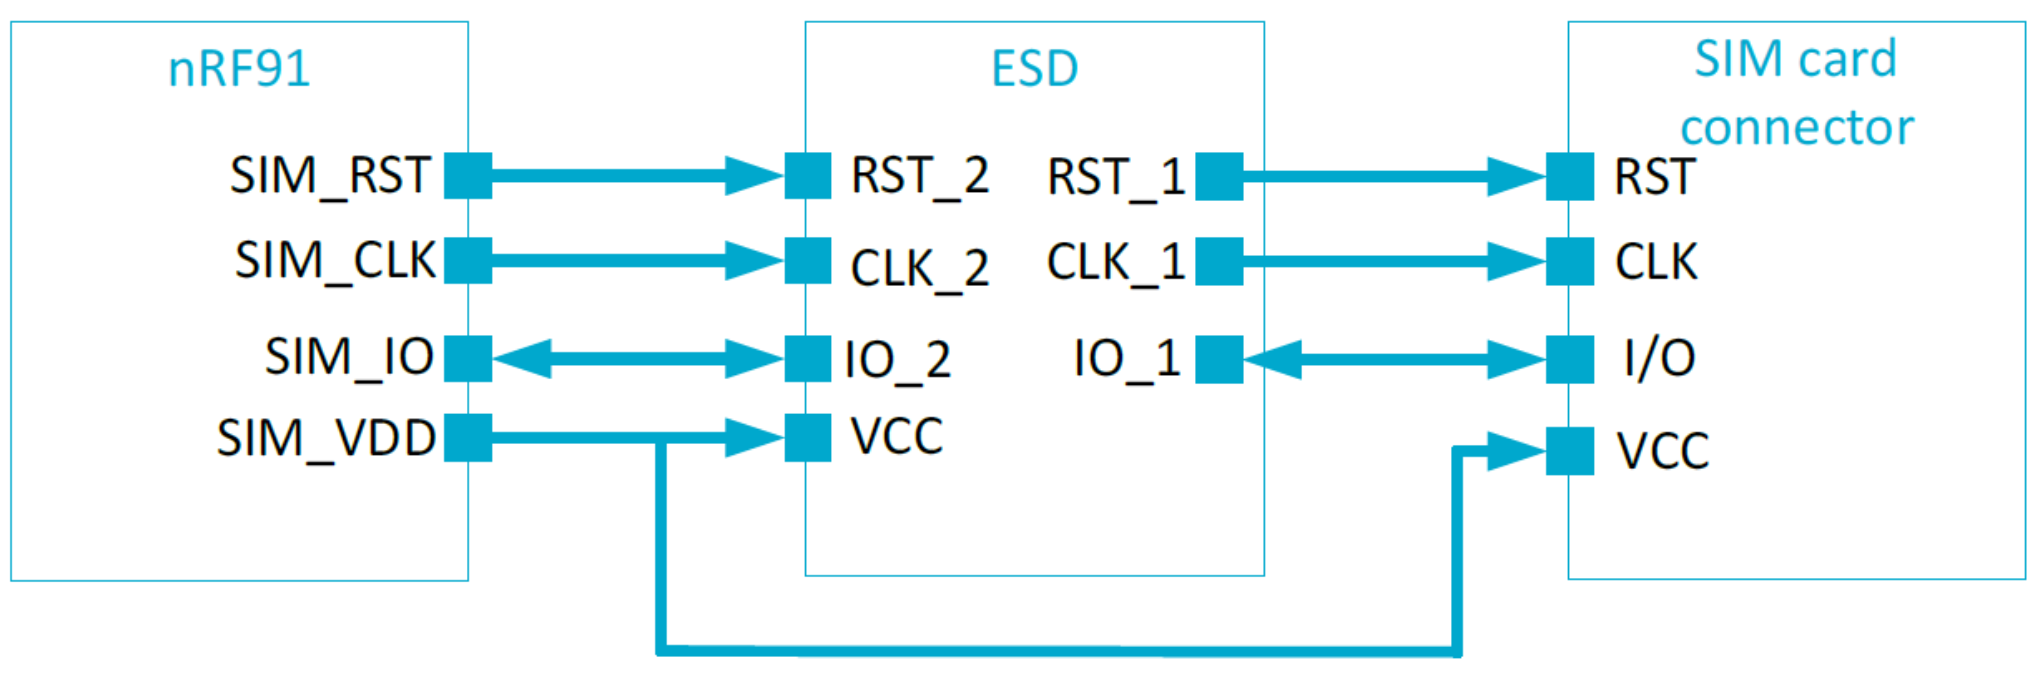
\includegraphics[width=1\textwidth]{Include/Figure/comp/nrf9160_sim_interf.png}
	\caption{Recommended Sim Card Interface Topology - Source:\cite{nRF9160}}
	\label{fig:nrf9160_sim_interf}
\end{figure}

The Sim card interface topology form \textsc{Nordi Semi} recommends interfacing the Sim card connector with the \textit{nRF9160} through an \textit{ESD} filter component to protect extremely sensitive inputs of the \textit{LTE} modem.

\pagebreak

According to the \textit{"Product Specification"}\cite{nRF9160} of the \textit{nRF9160}, the \textit{LTE} modem controls the physical interfaces towards the \textit{UICC} and implements the transport protocol over a four-pin \textit{ISO/IEC 7816-3} interface:
\begin{itemize}
\item VCC (power supply): LTE modem drives this
\item CLK (clock signal): LTE modem drives this
\item RST (reset signal): LTE modem drives this
\item I/O (input/output serial data): Bi-directional
\end{itemize}

\subsubsection{Accelerometer}

Figure \ref{fig:LTEWatch_nRF9160_Accelerometer} illustrates the electrical schematic of the \textit{MC3635} accelerometer:

\begin{figure}[H]
	\centering
	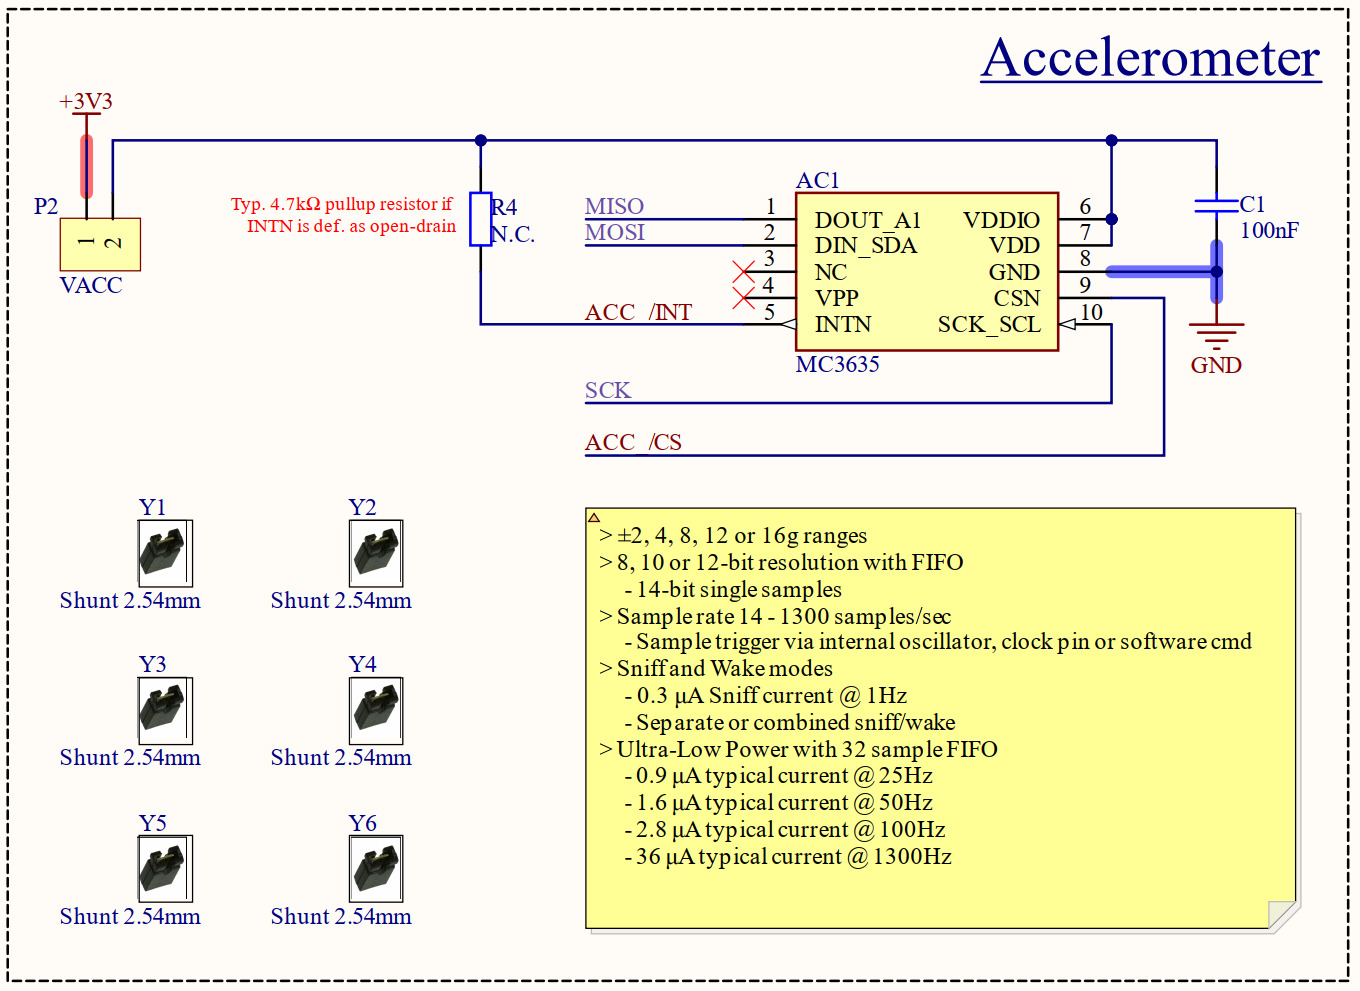
\includegraphics[width=1\textwidth]{Include/Figure/Hardware/LTEWatch_nRF9160_Accelerometer}
	\caption{nRF9160 : Accelerometer}
	\label{fig:LTEWatch_nRF9160_Accelerometer}
\end{figure}

The schematic shown in figure \ref{fig:LTEWatch_nRF9160_Accelerometer} is based on the typical 4-wire \textit{SPI} application circuit provided in the \textit{MC3635}\cite{MC3635} datasheet. More information about the accelerometer has already been presented on the page \pageref{sec:accl_sel}.


% ---------------------------- USER INT ----------------------------------
\pagebreak
\subsection{User interface}

TThis block concerns all functionality  related to the user interface.

\subsubsection{Buttons \& Switches}

Buttons and switch unit presented on the schematic of figure \ref{fig:LTEWatch_LTEW_User_Interface_Buttons_Switches} is based on the schematic from the \textit{nRF9160DK}\cite{nRF9160DK} board:

\begin{figure}[H]
	\centering
	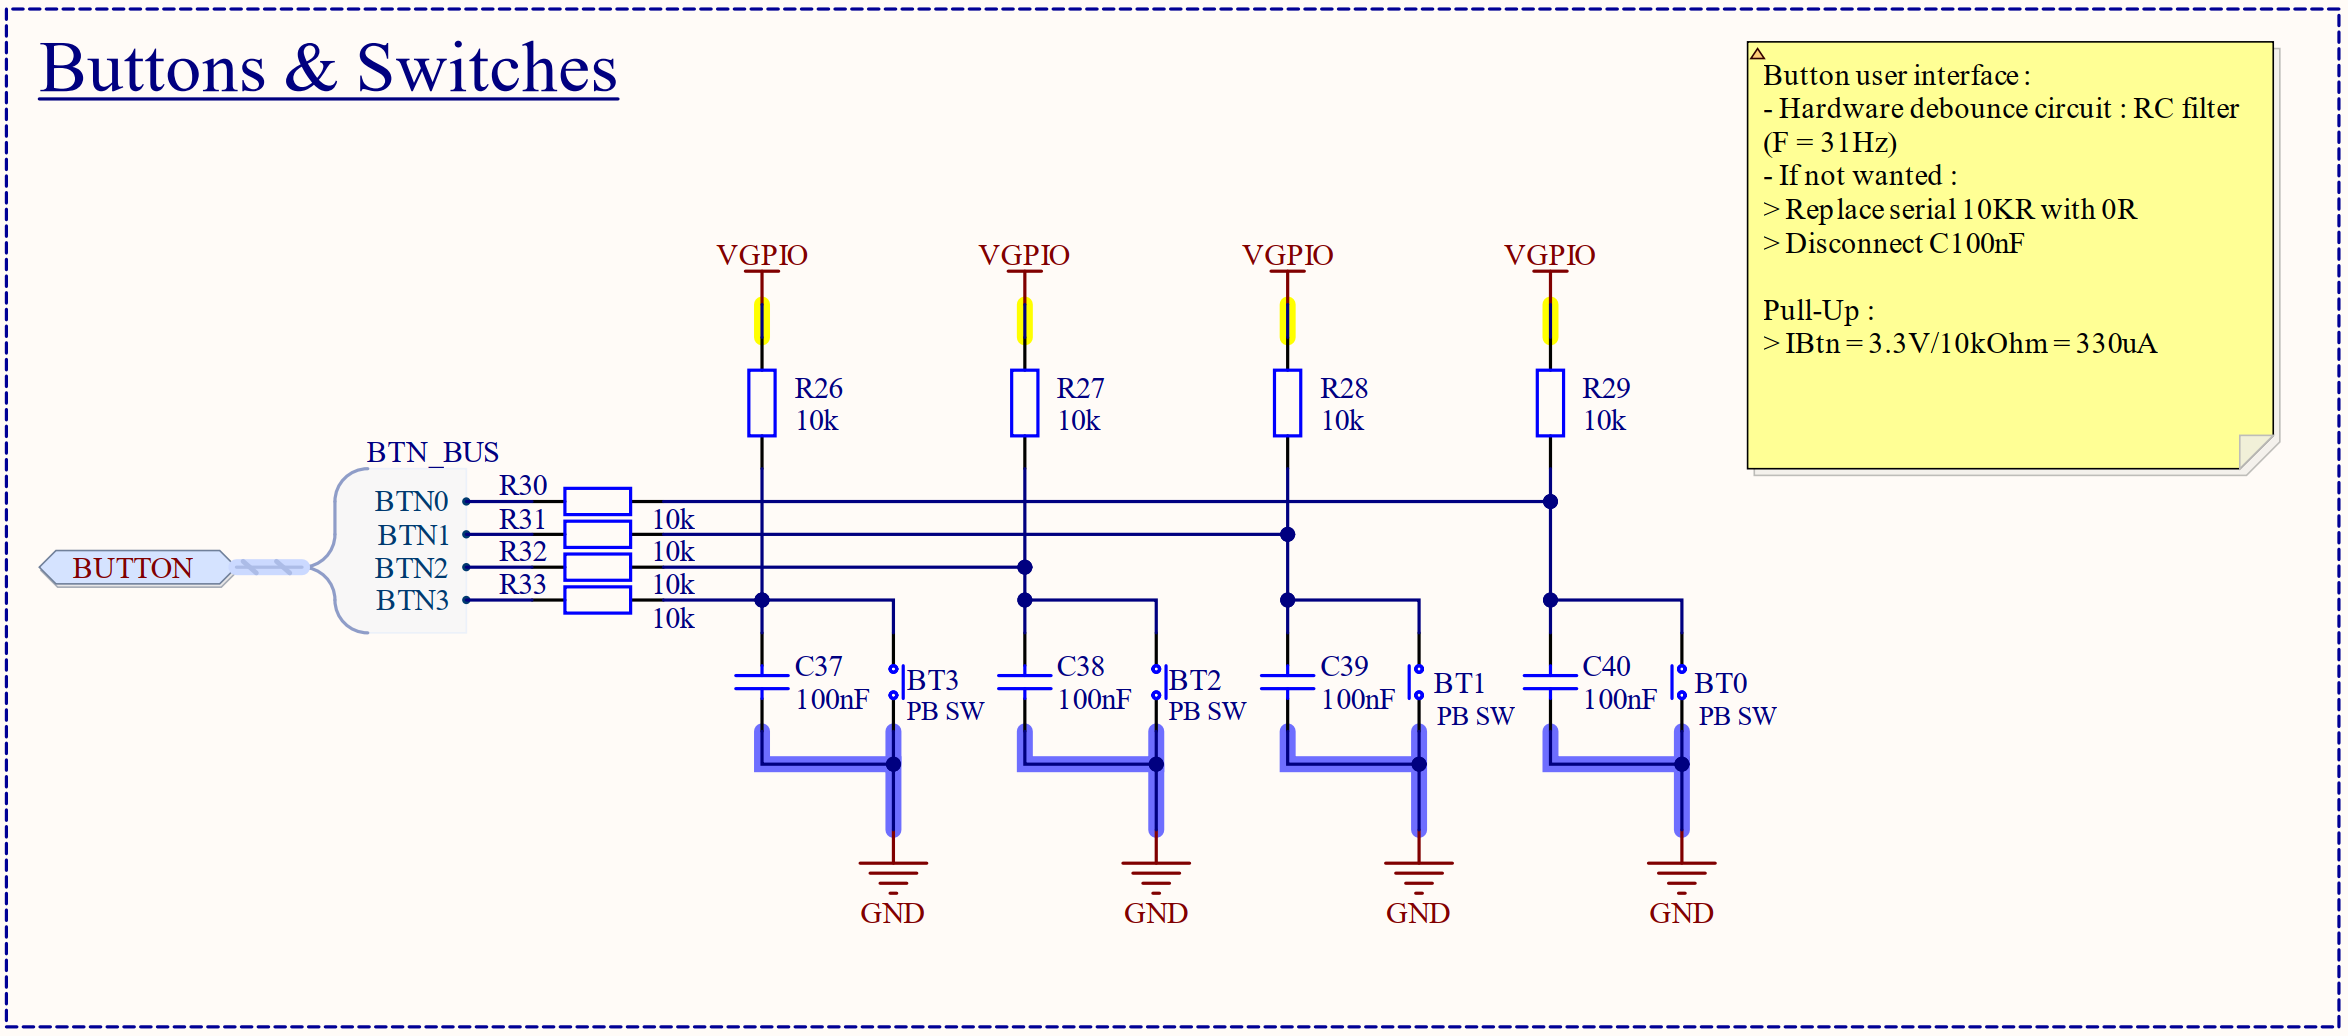
\includegraphics[width=1\textwidth]{Include/Figure/Hardware/LTEWatch_LTEW_User_Interface_Buttons_Switches}
	\caption{User Interface : Buttons \& Switches}
	\label{fig:LTEWatch_LTEW_User_Interface_Buttons_Switches}
\end{figure}

\subsubsection{Leds}

Leds unit presented on the schematic of figure \ref{fig:LTEWatch_LTEW_User_Interface_Leds} is based on the schematic from the \textit{nRF9160DK}\cite{nRF9160DK} board:

\begin{figure}[H]
	\centering
	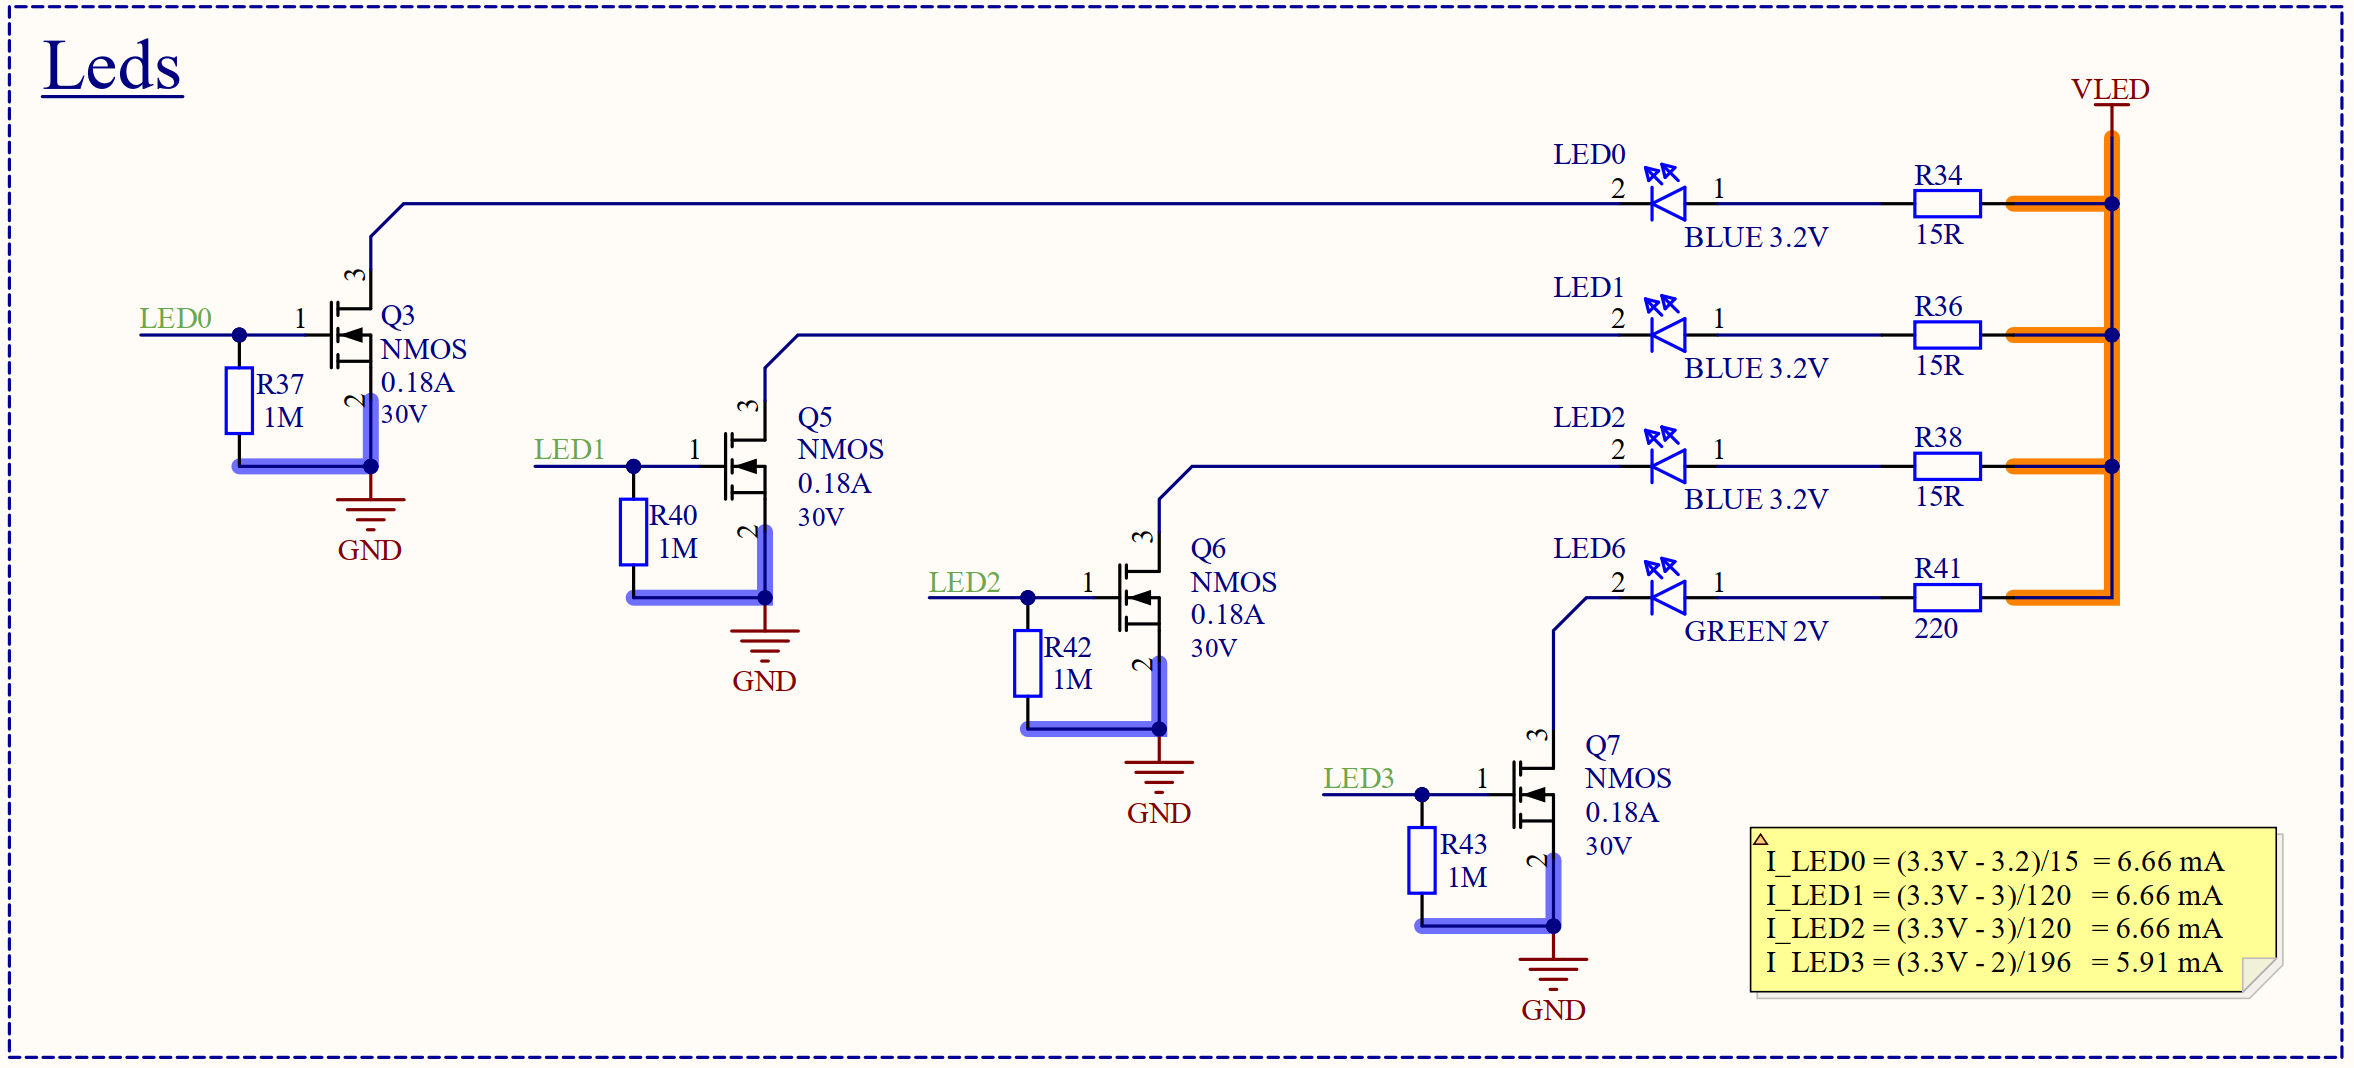
\includegraphics[width=1\textwidth]{Include/Figure/Hardware/LTEWatch_LTEW_User_Interface_Leds}
	\caption{User Interface : Leds}
	\label{fig:LTEWatch_LTEW_User_Interface_Leds}
\end{figure}



\subsubsection{Motors Driver}

Figure \ref{fig:LTEWatch_LTEW_User_Interface_Motors_Driver} illustrates the motor driver interface electrical schematic:

\begin{figure}[H]
	\centering
	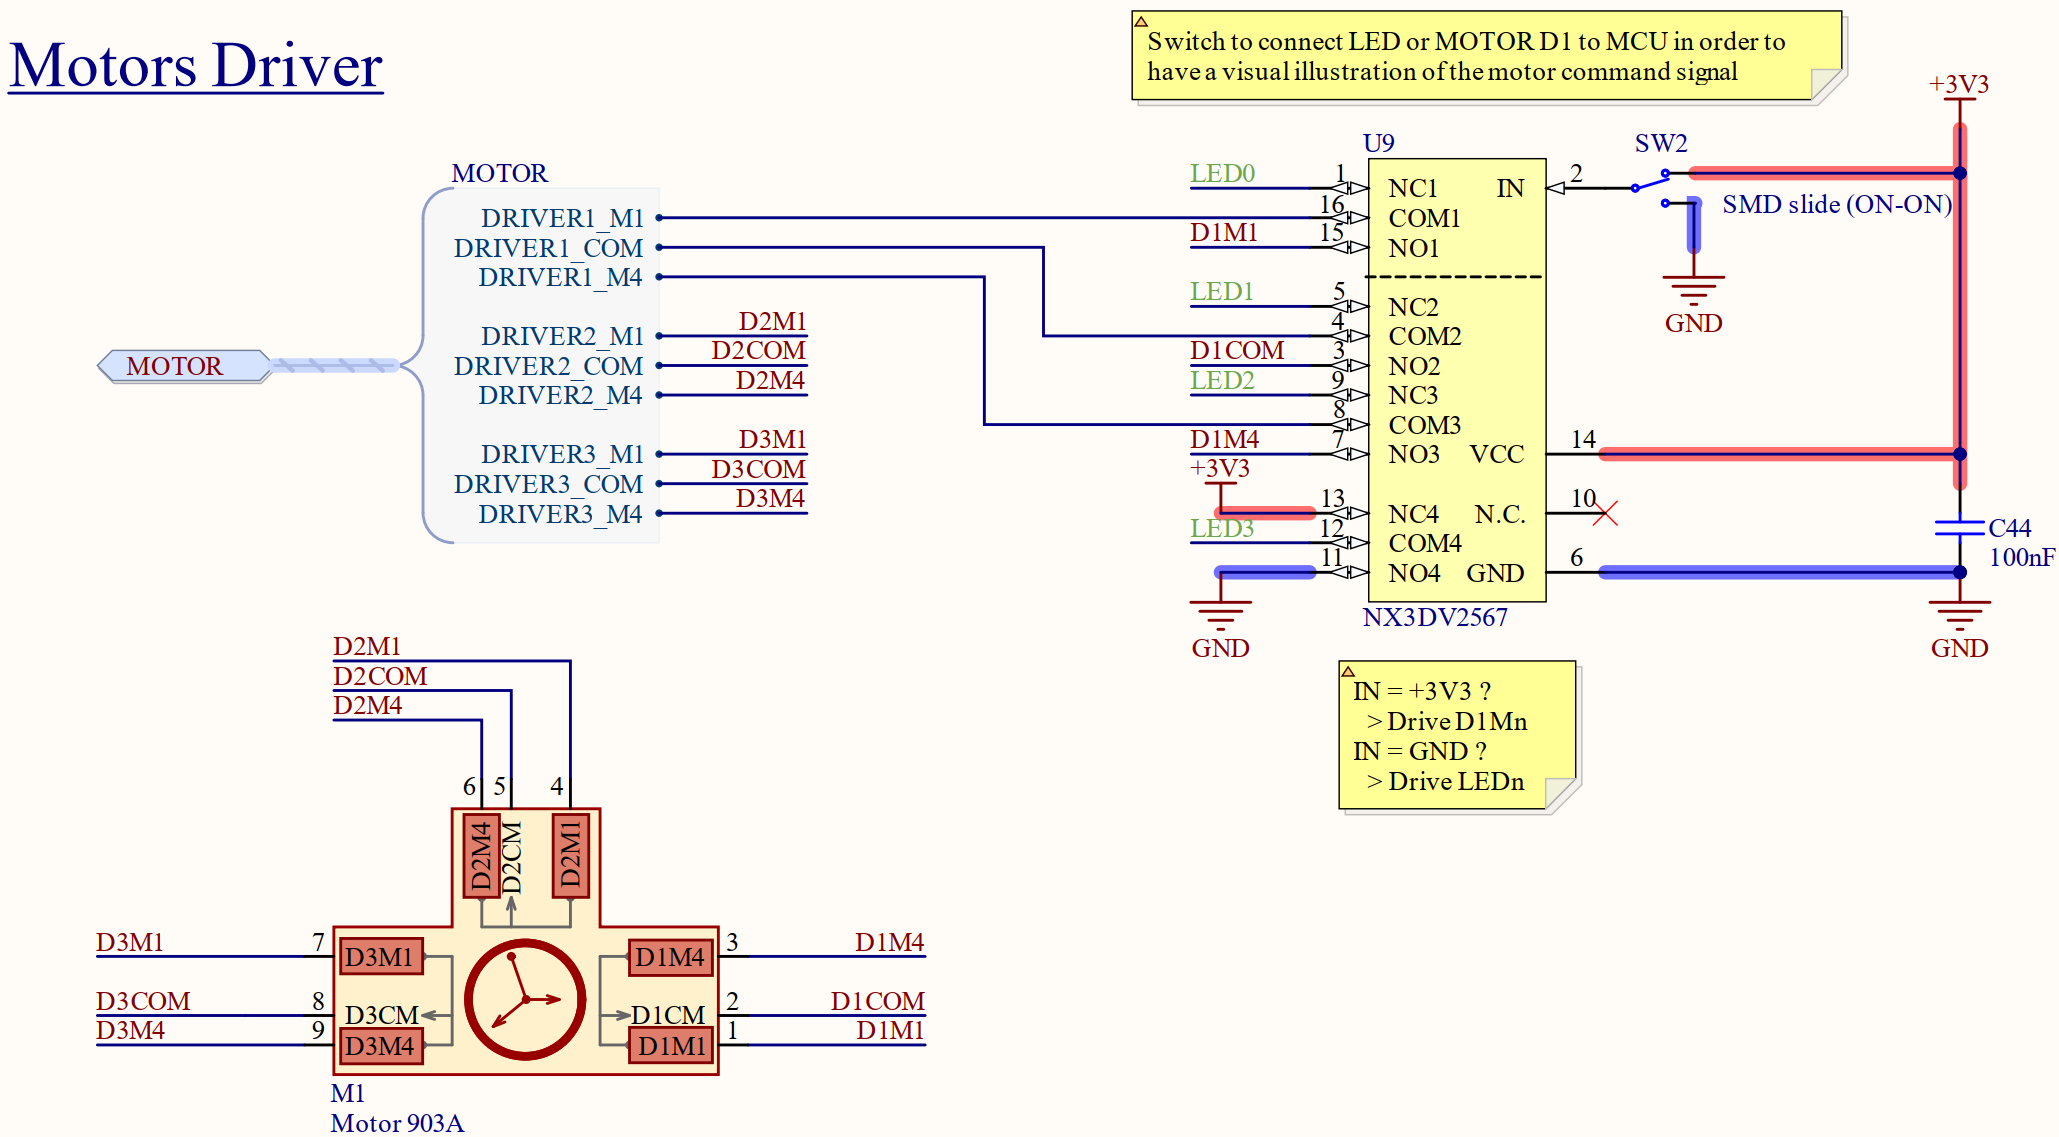
\includegraphics[width=1\textwidth]{Include/Figure/Hardware/LTEWatch_LTEW_User_Interface_Motors_Driver}
	\caption{User Interface : Motors Driver}
	\label{fig:LTEWatch_LTEW_User_Interface_Motors_Driver}
\end{figure}

The schematic shown at \ref{fig:LTEWatch_LTEW_User_Interface_Motors_Driver} contains the motor drive pin connectors and the parallel switch that allows three signals from the motor driver to be redirected to three external LEDs for debugging purposes.

\subsubsection{Display Interface}

The electrical schematics relatives to the display interface are shown in figures \ref{fig:LTEWatch_LTEW_User_Interface_Filter_Power_Supply} to \ref{fig:LTEWatch_LTEW_User_Interface_NiceViewConnector}:

\begin{figure}[H]
	\centering
	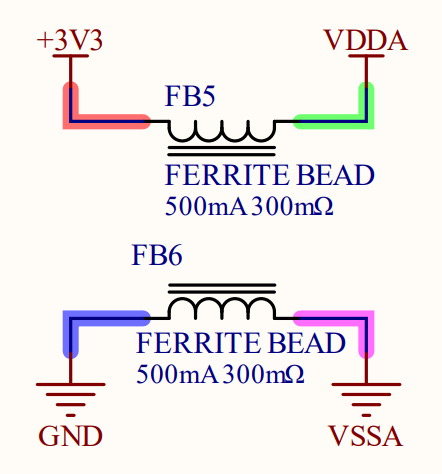
\includegraphics[width=0.4\textwidth]{Include/Figure/Hardware/LTEWatch_LTEW_User_Interface_Filter_Power_Supply}
	\caption{User Interface : Display Interface - Power Supply Filter}
	\label{fig:LTEWatch_LTEW_User_Interface_Filter_Power_Supply}
\end{figure}

\begin{figure}[H]
	\centering
	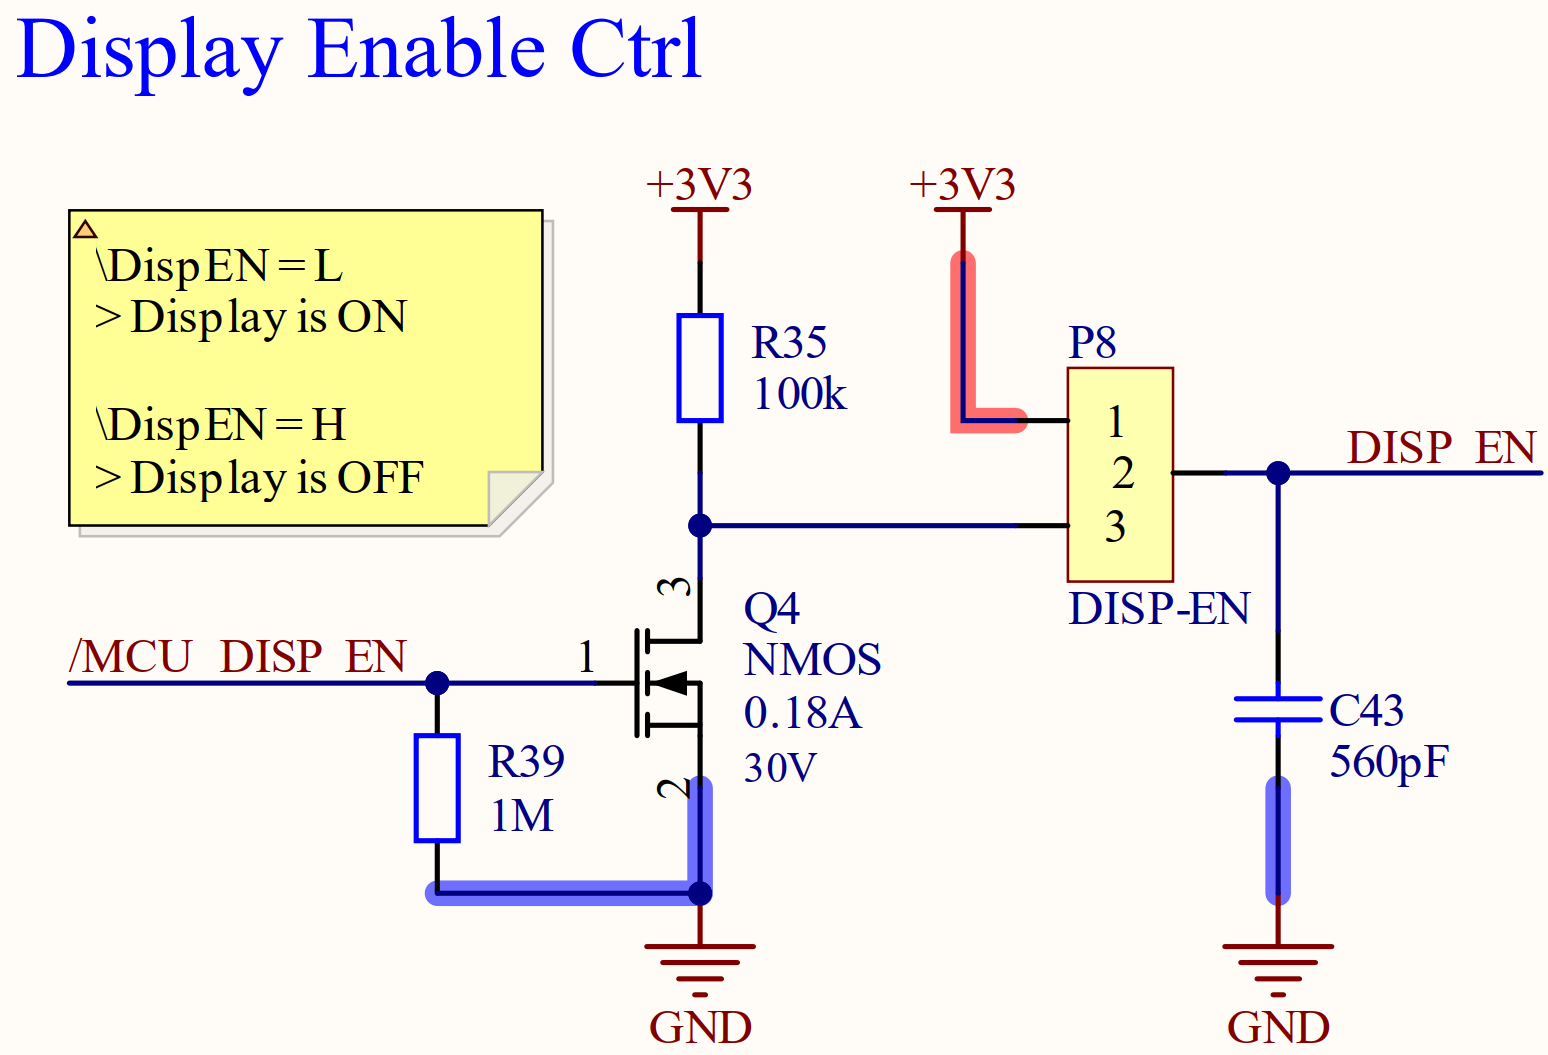
\includegraphics[width=0.7\textwidth]{Include/Figure/Hardware/LTEWatch_LTEW_User_Interface_Display_En_CTRL}
	\caption{User Interface : Display Interface - Display Enable}
	\label{fig:LTEWatch_LTEW_User_Interface_Display_En_CTRL}
\end{figure}

\begin{figure}[H]
	\centering
	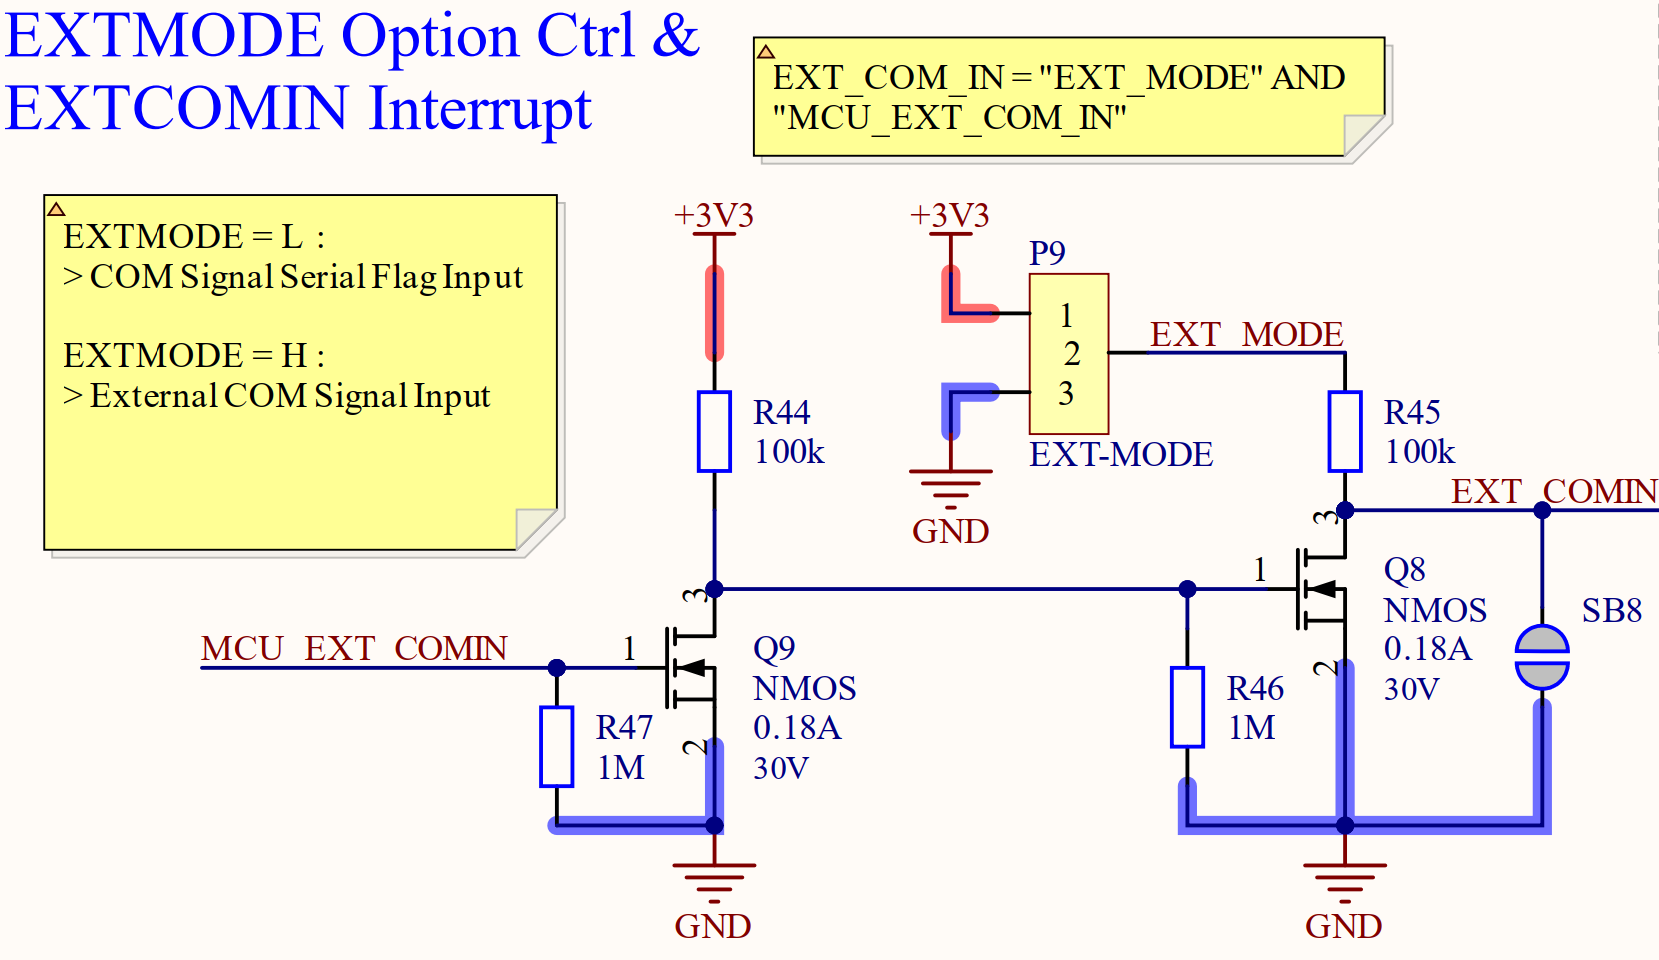
\includegraphics[width=0.9\textwidth]{Include/Figure/Hardware/LTEWatch_LTEW_User_Interface_EXTMODE}
	\caption{User Interface : Display Interface - EXTMODE Control}
	\label{fig:LTEWatch_LTEW_User_Interface_EXTMODE}
\end{figure}

\begin{figure}[H]
	\centering
	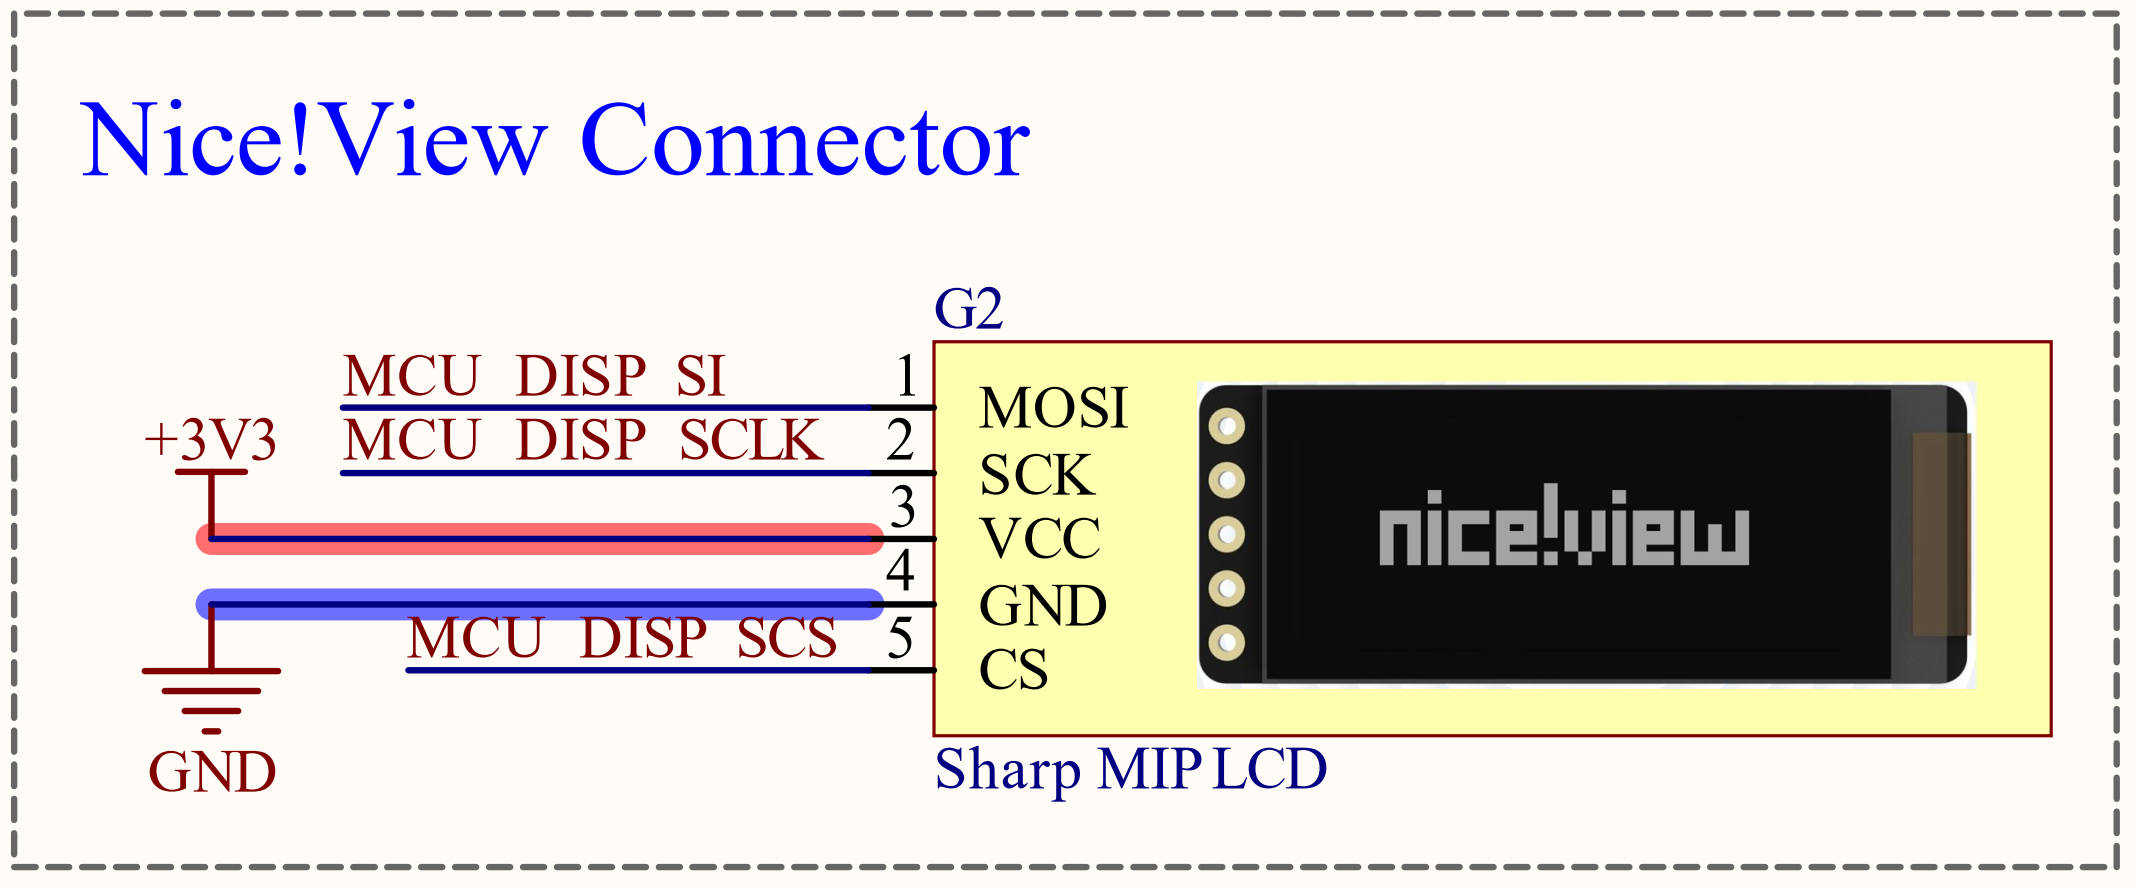
\includegraphics[width=0.7\textwidth]{Include/Figure/Hardware/LTEWatch_LTEW_User_Interface_NiceViewConnector}
	\caption{User Interface : Display Interface - \textit{nice!view} Connector}
	\label{fig:LTEWatch_LTEW_User_Interface_NiceViewConnector}
\end{figure}


\begin{figure}[H]
	\centering
	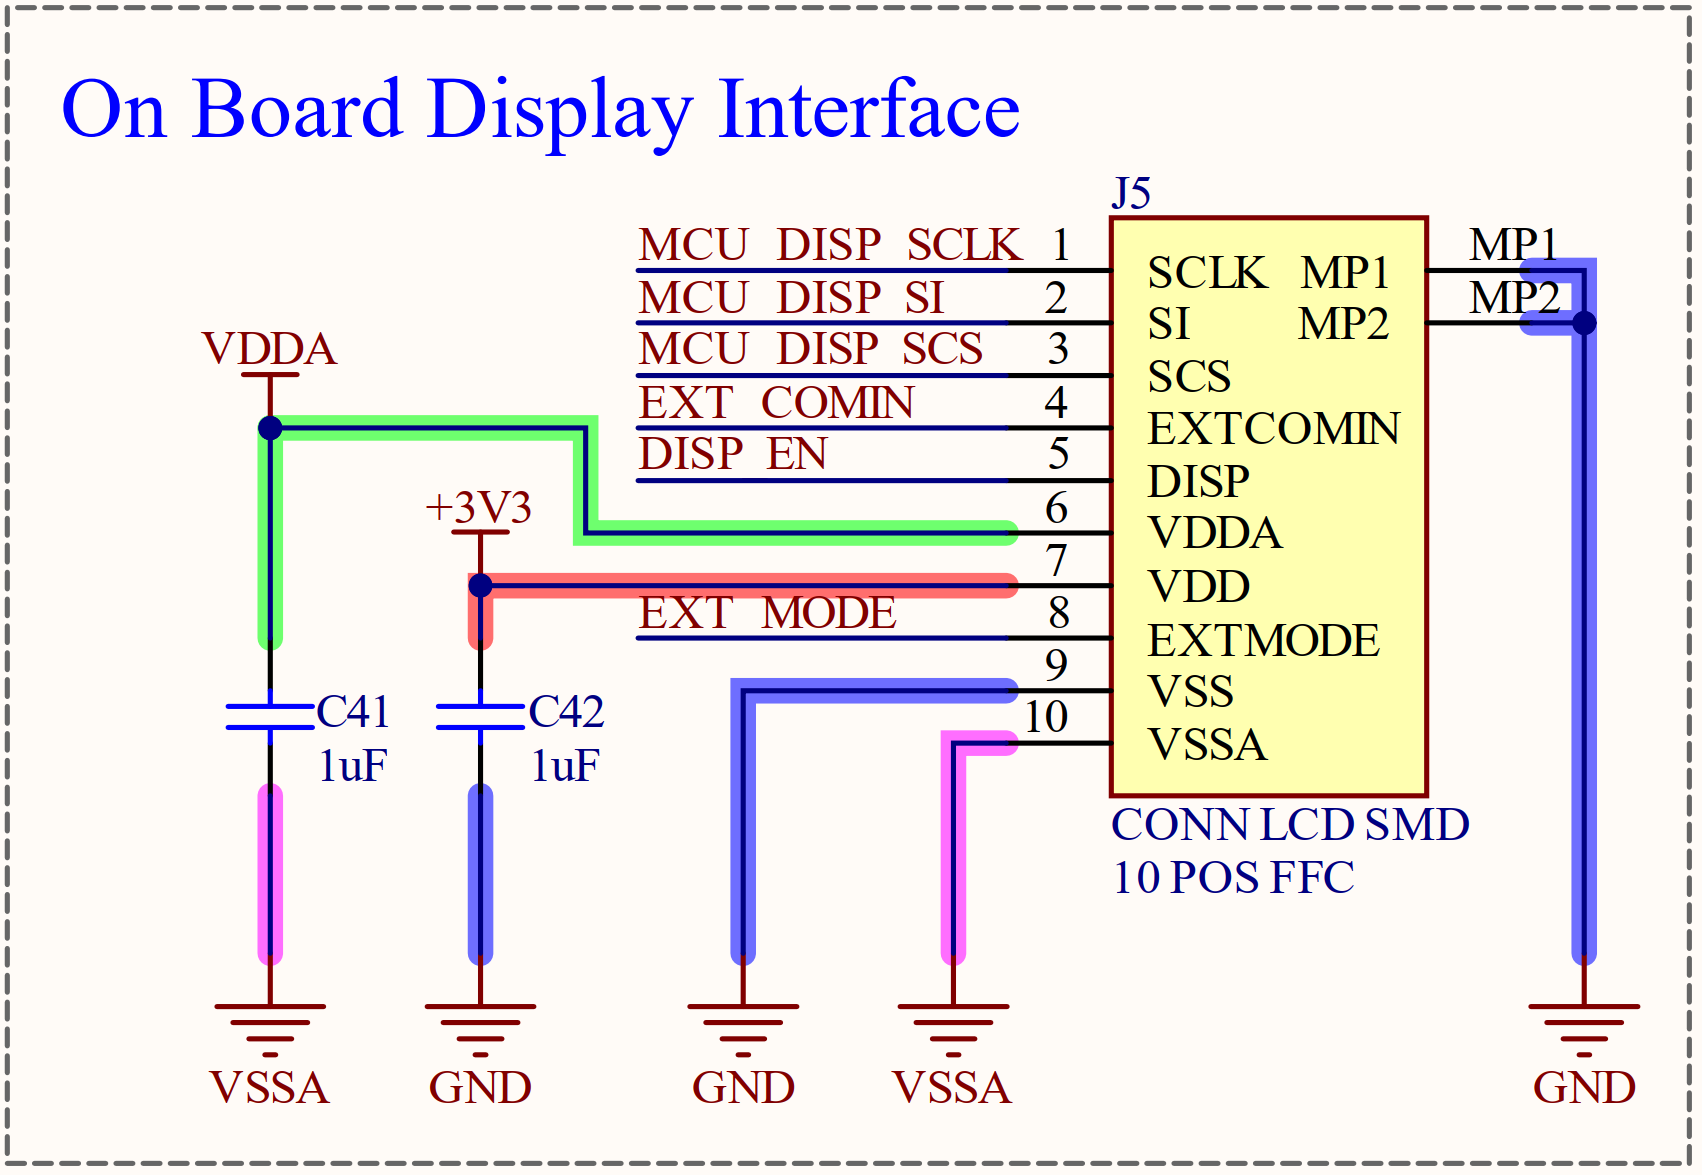
\includegraphics[width=0.8\textwidth]{Include/Figure/Hardware/LTEWatch_LTEW_User_Interface_OnBoard_Dsp_Interface}
	\caption{User Interface : Display Interface - Display Interface}
	\label{fig:LTEWatch_LTEW_User_Interface_OnBoard_Dsp_Interface}
\end{figure}

% ------------------------------ RF UNIT ---------------------------------

\subsection{RF Unit (Radio Freq)}
This contains all units and module relative to RF signals transmission, such as:
\begin{itemize}
\item GNSS Receiver
\item GNSS Enable
\item GNSS RF Transmission Line
\item GPS Contolled by MCU or Ext 
\item LTE RF transmission Line
\end{itemize}

\subsubsection{GNSS Enable}

Figure \ref{fig:LTEWatch_LTEW_RF_Unit_GPS_Enable} illustrates the \textit{GNSS} Enable circuit schematic:

\begin{figure}[H]
	\centering
	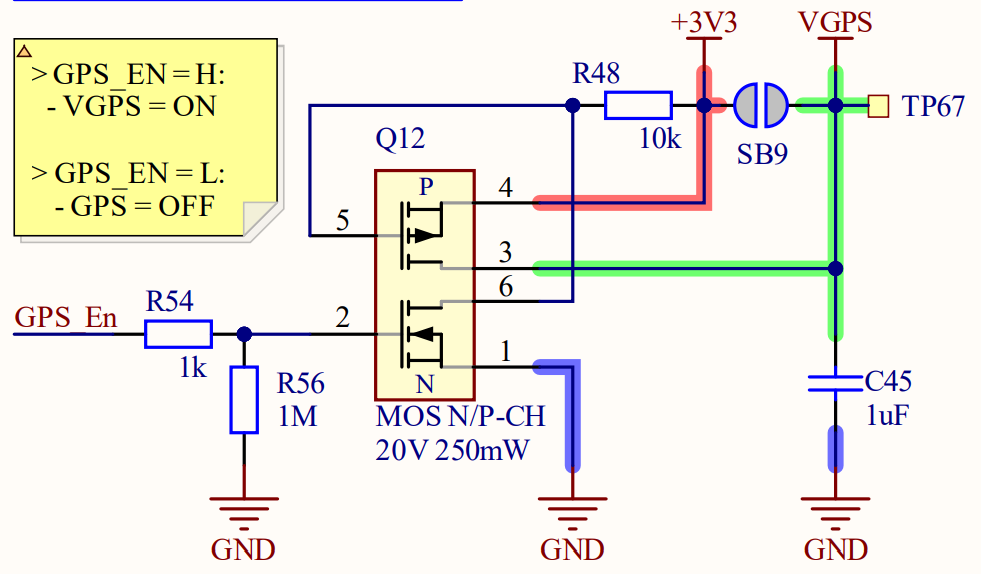
\includegraphics[width=0.7\textwidth]{Include/Figure/Hardware/LTEWatch_LTEW_RF_Unit_GPS_Enable}
	\caption{RF Unit : GNSS Enable}
	\label{fig:LTEWatch_LTEW_RF_Unit_GPS_Enable}
\end{figure}


\subsubsection{GNSS Receiver}

Figure \ref{fig:LTEWatch_LTEW_RF_Unit_GNSS_Receiver} illustrate the electrical schematic of the integration of the GNSS receiver \textit{MAX-M10S} from \textsc{u-blox}:

\begin{figure}[H]
	\centering
	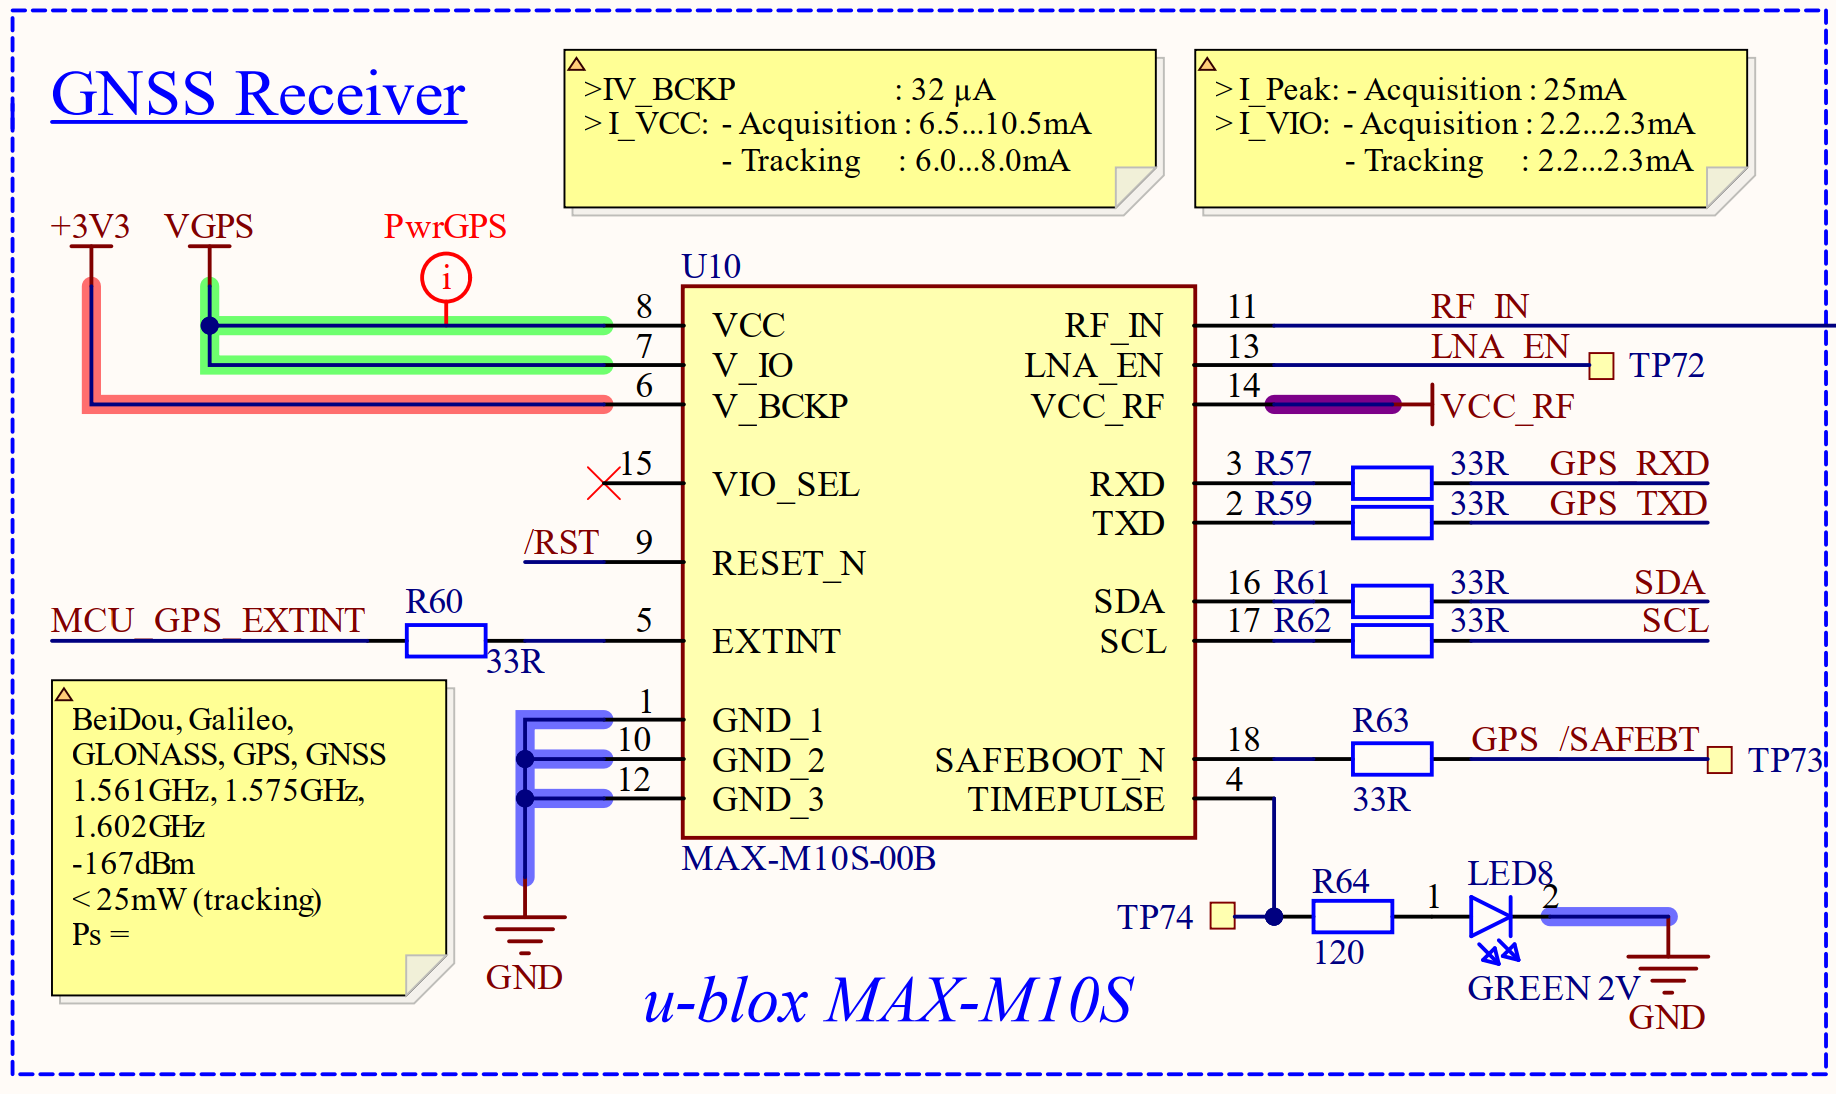
\includegraphics[width=1\textwidth]{Include/Figure/Hardware/LTEWatch_LTEW_RF_Unit_GNSS_Receiver}
	\caption{RF Unit : GNSS Receiver \textit{MAX-M10S}}
	\label{fig:LTEWatch_LTEW_RF_Unit_GNSS_Receiver}
\end{figure}

The schematic shown in figure \ref{fig:LTEWatch_LTEW_RF_Unit_GNSS_Receiver} is based on the open source schematic of "\textit{GNSS Receiver Breakout - MAX-M10S (Qwiic)}" from \textsc{Sparkfun}: \url{https://www.sparkfun.com/products/18037}. The main difference is that I added the possibility to either use the \textit{GNSS} receiver with an on-board chip antenna or with an external antenna that can be connected through a \textit{SMA} connector. Except that, the integration is fairly simple with only some series resistors added on each lines to limit currents.\\

On \textit{the LTEWatch}, the \textit{GNSS} receiver can be power or not in order to keep a better control on system consumption and battery life. The \textit{GNSS} is powered through a dual MOSFET non-inverting switch that connect the \textit{VCC} and \textit{V\_IO} pin of the \textit{GNSS} receiver to the board \SI{3.3}{\volt} when GOS\_En is set \textit{'high'}.\\

The \textit{V\_BCKP} pin of the \textit{GNSS} receiver is directly connected to the \SI{3.3}{\volt} to enable the hardware backup mode, which reduces the \textit{TTFF} and consumption of the \textit{GNSS} receiver module.

\pagebreak
\subsubsection{GNSS RF Transmission Line}

Figuer \ref{fig:LTEWatch_LTEW_RF_Unit_RF_Switch} illustrates the schematic of the \textit{GNSS} RF line (front-end):

\begin{figure}[H]
	\centering
	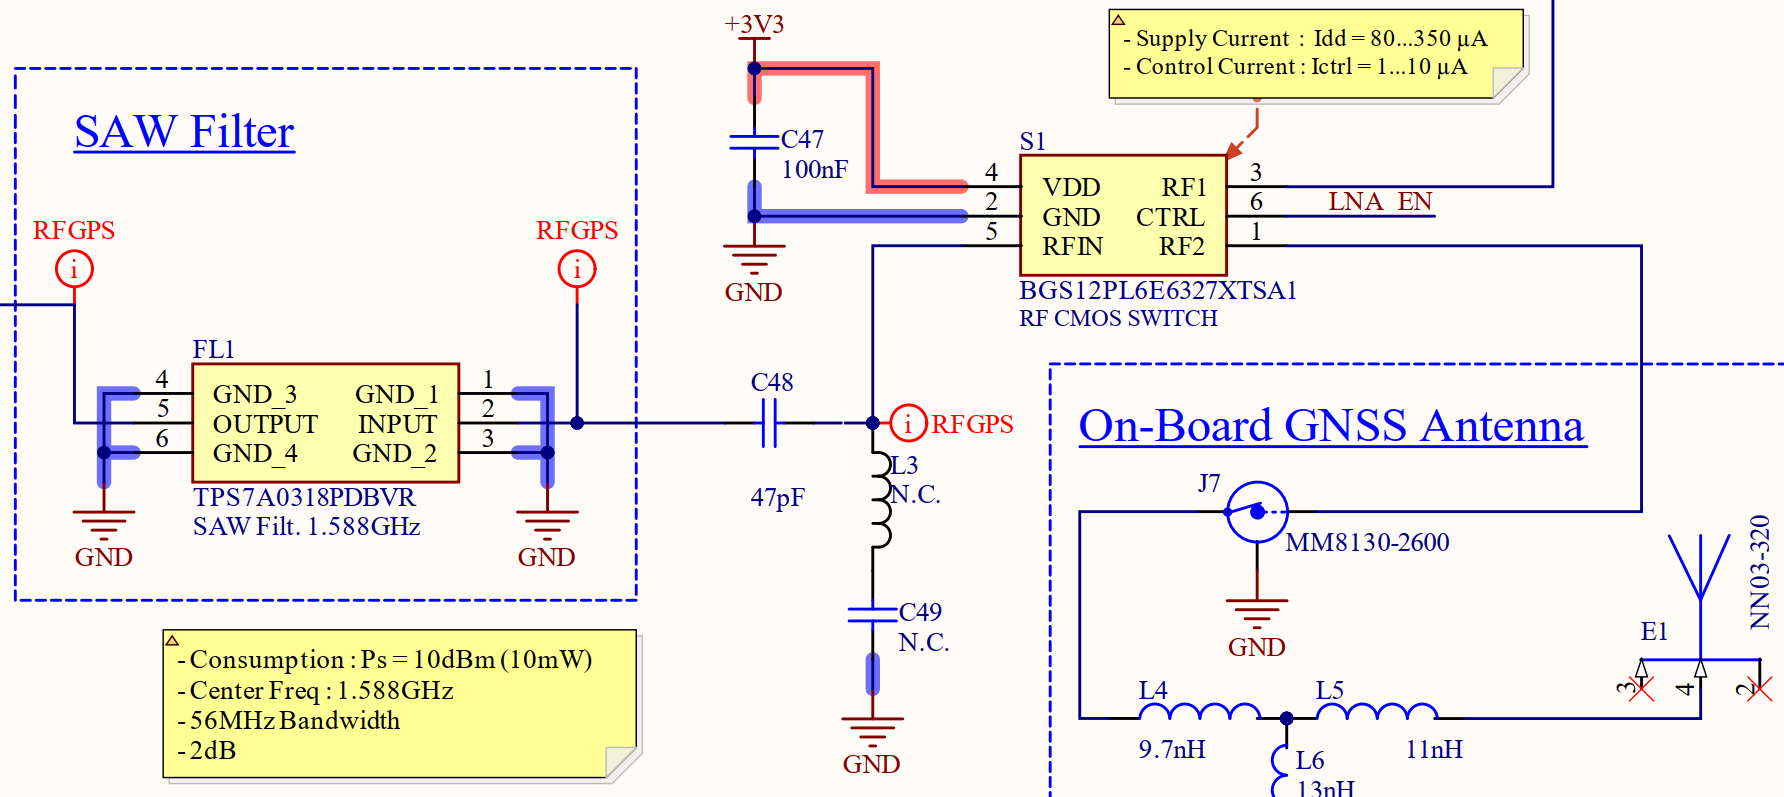
\includegraphics[width=1\textwidth]{Include/Figure/Hardware/LTEWatch_LTEW_RF_Unit_RF_Switch}
	\caption{RF Unit : RF Switch with \textit{SAW} Filter}
	\label{fig:LTEWatch_LTEW_RF_Unit_RF_Switch}
\end{figure}

In order to add the possibility to connect the \textit{GNSS} receiver to the on-board chip antenna or to an external active antenna, a RF switch is added. The RF switch is a \textit{BGS12PL6E6327}\cite{BGS12PL6}, which is a general purpose RF \textit{CMOS} \textit{SPDT} switch with the following specifications (src.\cite{BGS12PL6}):
\begin{itemize}
\item 2 high-linearity TRx paths with power handling capability of up to 35 dBm
\item All ports are fully symmetrical
\item Low insertion loss
\item Low harmonic generation
\item High port-to-port isolation
\item 30 MHz to 4 GHz coverage
\item High ESD robustness
\item On-chip control logic
\item No decoupling capacitors required if no DC applied on RF lines\\
\end{itemize}

To add more robustness against interference and following the design recommendations that were presented on page \pageref{sec:gnss_rcvr_sel}, an addition external SAW filter is implemented right before the front-end of the \textit{GNSS} receiver. This seems necessary, due to the presence of both \textit{GNSS} and \textit{LTE} antenna present on the same board.\\

\pagebreak

Figure \ref{fig:LTEWatch_LTEW_RF_Unit_Ext_GNSS_Antenna} illustrates the schematic of the \textit{GNSS} external antenna power supply supervisor:

\begin{figure}[H]
	\centering
	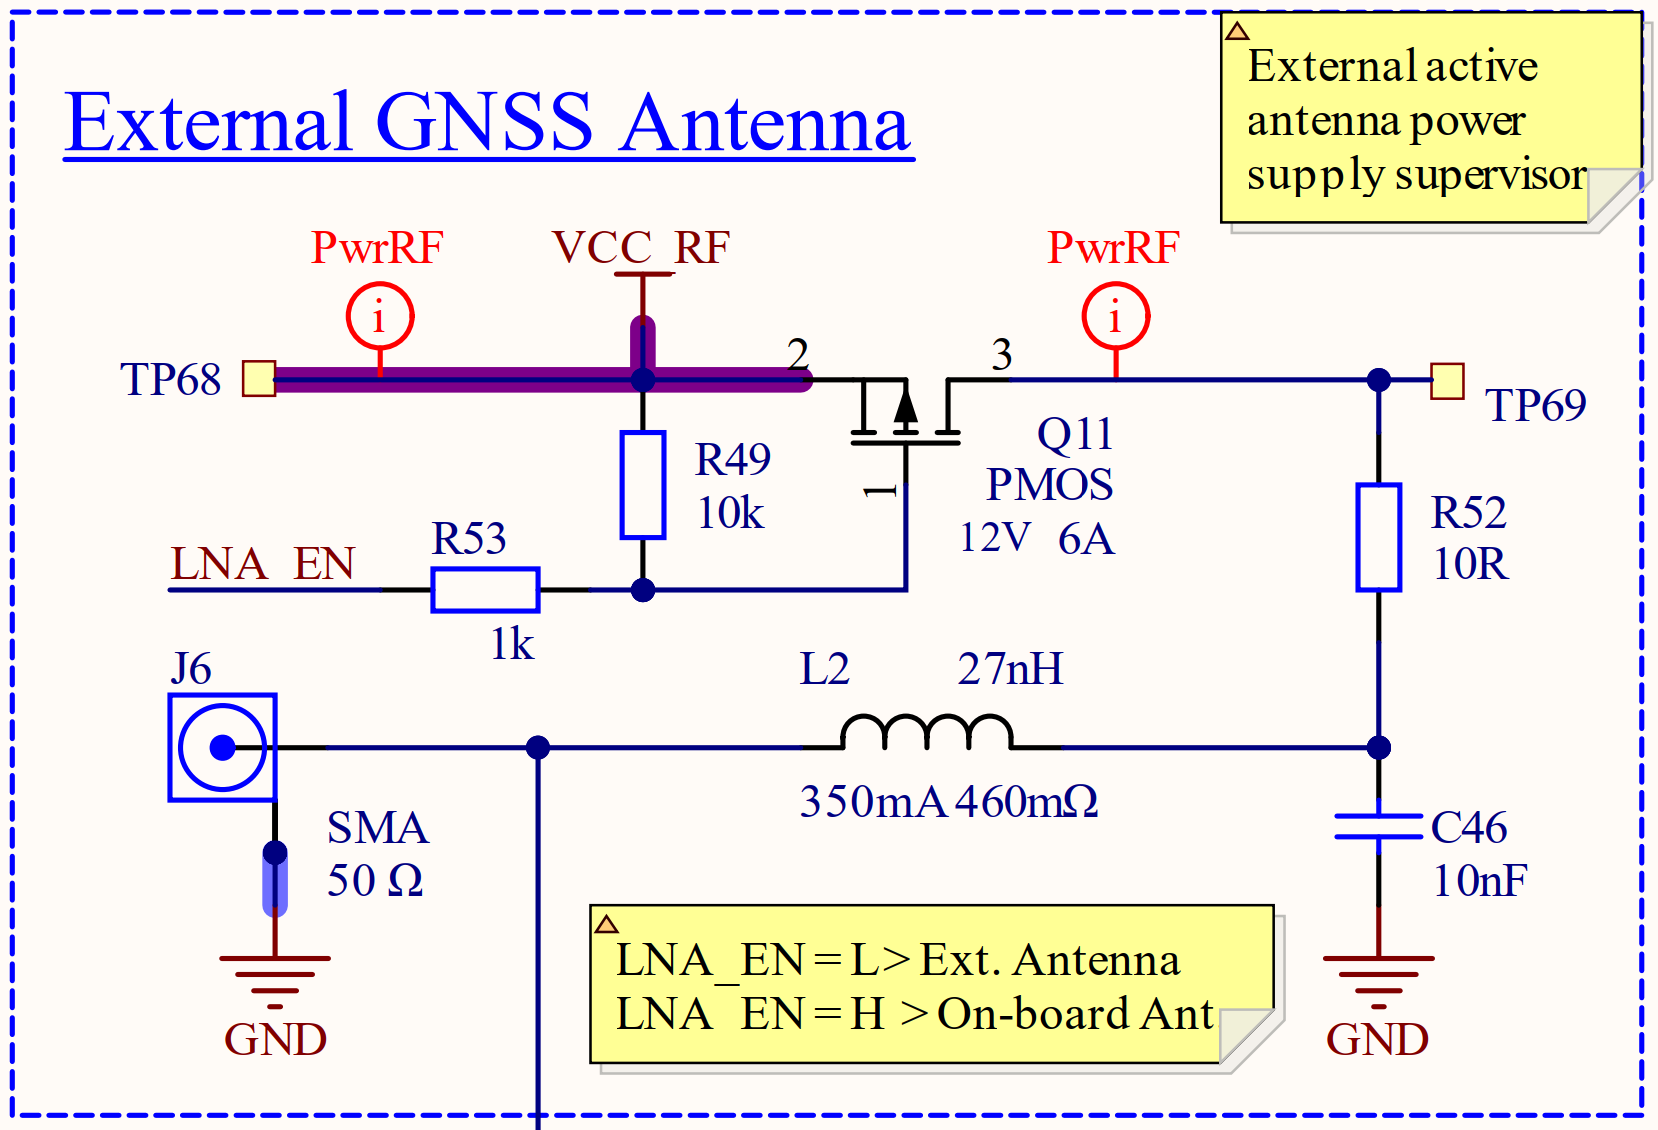
\includegraphics[width=0.65\textwidth]{Include/Figure/Hardware/LTEWatch_LTEW_RF_Unit_Ext_GNSS_Antenna}
	\caption{RF Unit : External GNSS Antenna}
	\label{fig:LTEWatch_LTEW_RF_Unit_Ext_GNSS_Antenna}
\end{figure}

The external \textit{GNSS} antenna power supply supervisor is based on the "\textit{MAX-M10S two-pin antenna supervisor}" application diagram from the integration manual of the \textit{MAX-M10S}\cite{MAXM10SINT}. When the LNA\_EN signal from the \textit{MAX-M10S} is set 'low' (internal \textit{LNA} mode configuration) the antenna power supply source \textit{VCC\_RF} is connected to the RF line and the \textit{SMA} connector to the supply in order to power an external active \textit{GNSS} antenna.\\

Figure \ref{fig:LTEWatch_LTEW_RF_Unit_OnBoard_GNSS_Antenna} illustrates the schematic of the on-board GNSS chip antenna which is the \textit{NN03-320} model from \textsc{ignion}. The advantage with this company, is that they furnish simulation and component tuning values for custom board for free. To make the design process faster and to try it out, I used the components value that they recommended for my board. The full simulation and documentation from \textsc{ignion} is in appendix \ref{appendix:LTEWatch_NNS1}.

\begin{figure}[H]
	\centering
	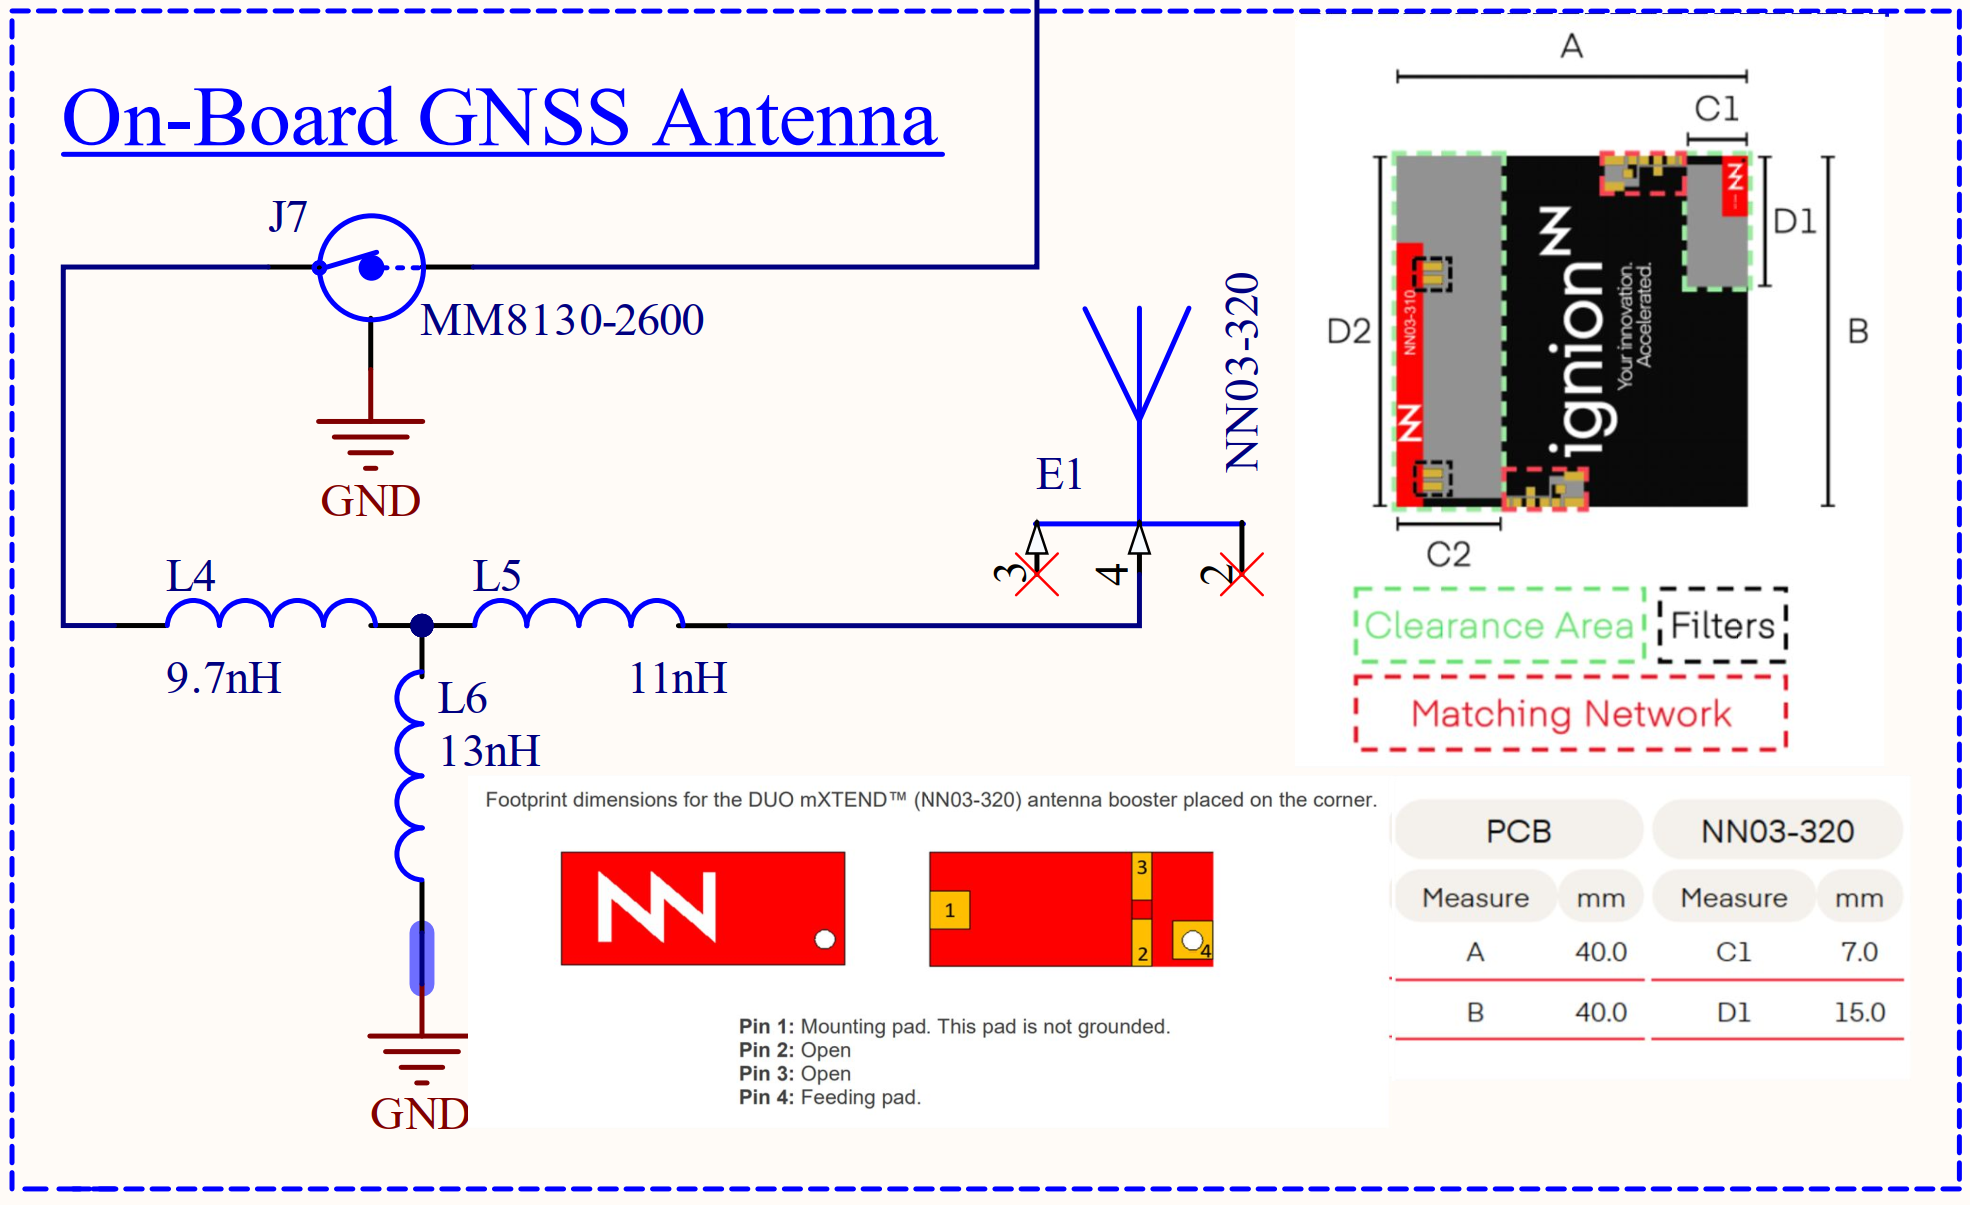
\includegraphics[width=0.7\textwidth]{Include/Figure/Hardware/LTEWatch_LTEW_RF_Unit_OnBoard_GNSS_Antenna}
	\caption{RF Unit : On Board GNSS Antenna}
	\label{fig:LTEWatch_LTEW_RF_Unit_OnBoard_GNSS_Antenna}
\end{figure}

\subsubsection{GPS Ctrl MCU/Ext}

Figure \ref{fig:LTEWatch_LTEW_RF_Unit_GPS_Ctrl_MCU-EXT} illustrate schematic of \textit{GNSS} \textit{UART}
bus configuration:

\begin{figure}[H]
	\centering
	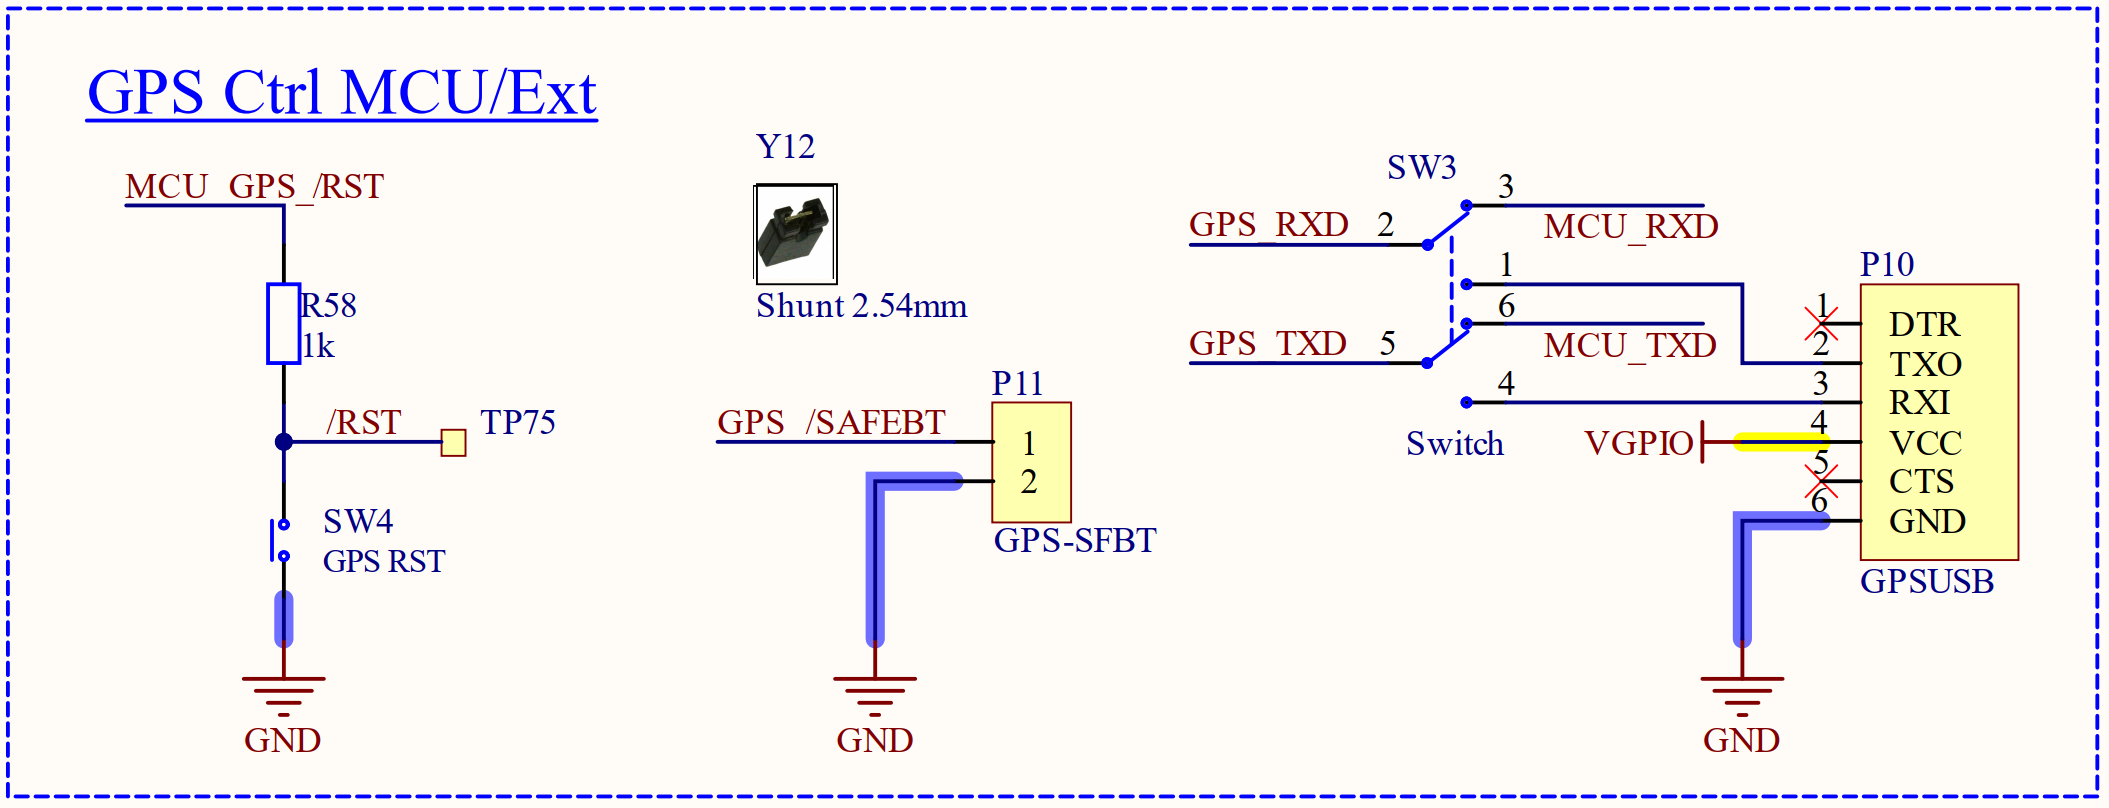
\includegraphics[width=1\textwidth]{Include/Figure/Hardware/LTEWatch_LTEW_RF_Unit_GPS_Ctrl_MCU-EXT}
	\caption{RF Unit : GPS External/MCU Control Selection}
	\label{fig:LTEWatch_LTEW_RF_Unit_GPS_Ctrl_MCU-EXT}
\end{figure}

This unit allows to connect the \textit{UART} of the \textit{GNSS} receiver to an external \textit{UART} interface or to the system \textit{MCU} (nRF9160). 

\subsubsection{LTE RF Transmission Line}

Figure \ref{fig:LTEWatch_LTEW_RF_Unit_Cellular_LTE_Antenna_Interface} illustrated the schematic of the LTE RF transmission line:

\begin{figure}[H]
	\centering
	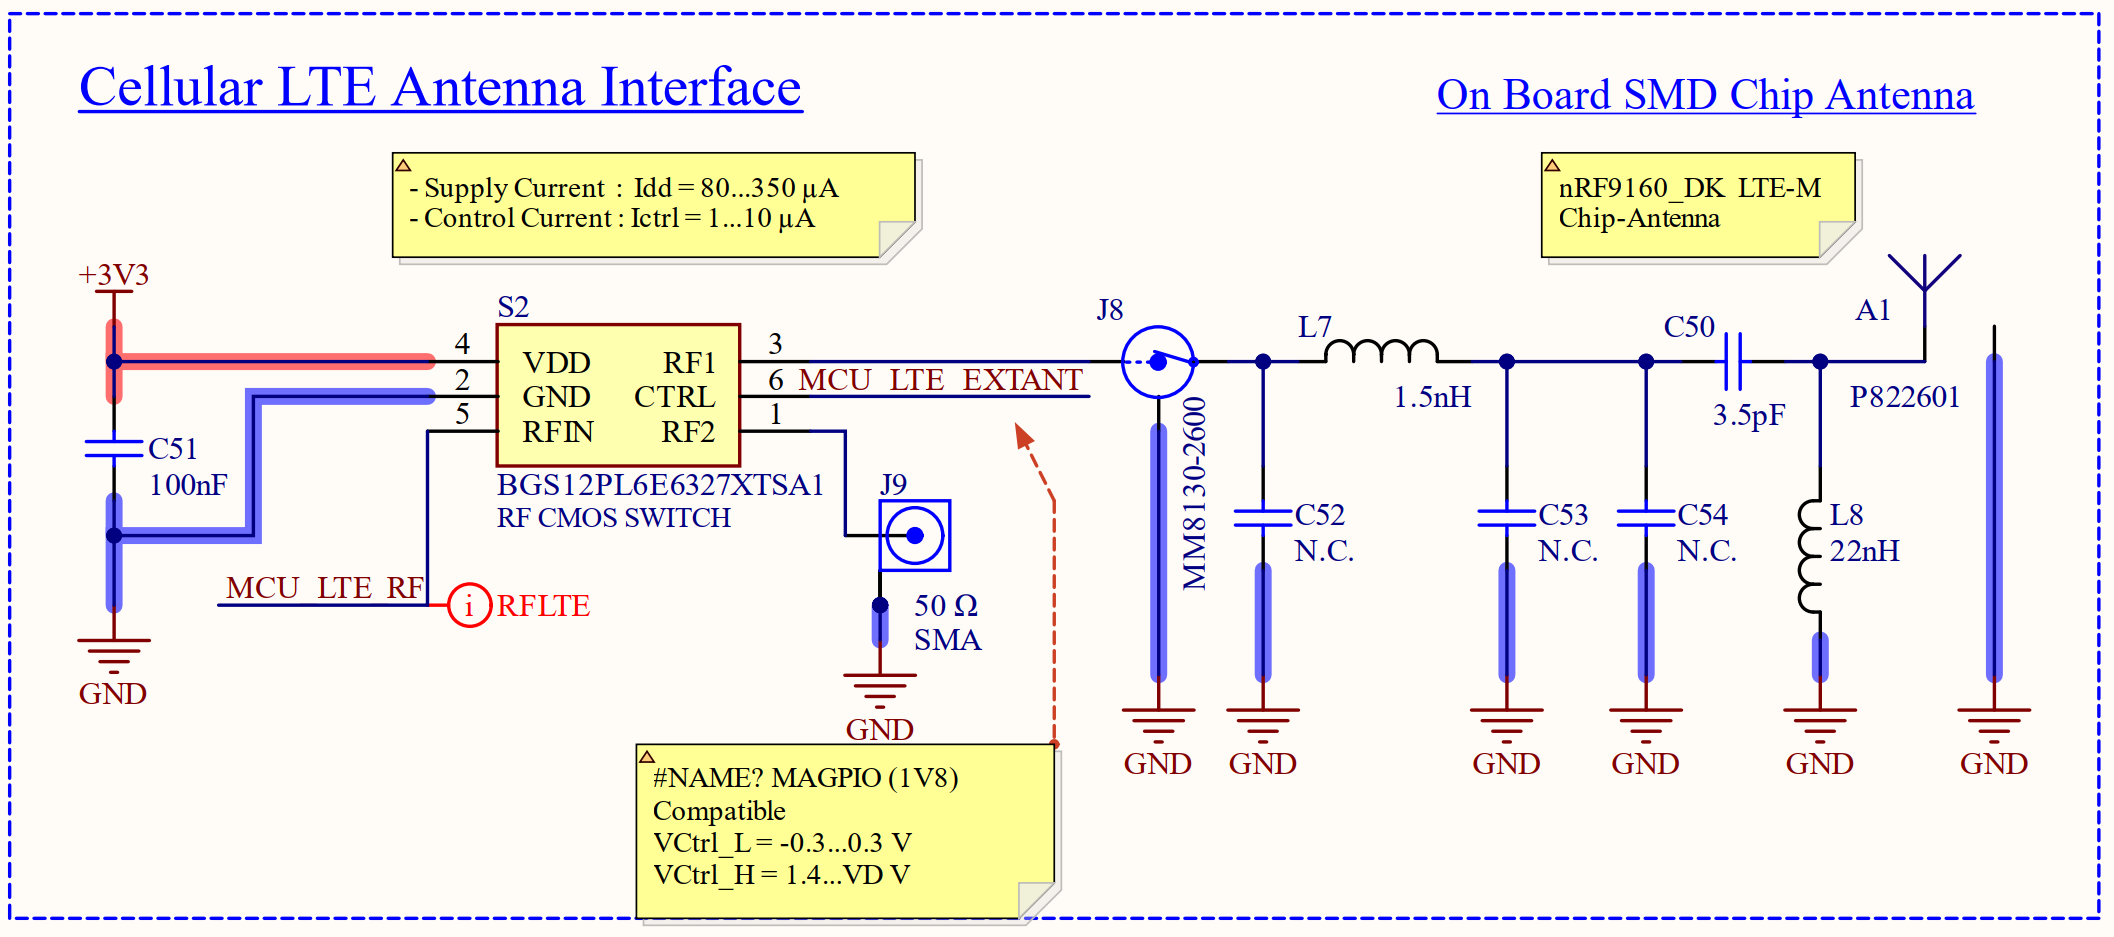
\includegraphics[width=1\textwidth]{Include/Figure/Hardware/LTEWatch_LTEW_RF_Unit_Cellular_LTE_Antenna_Interface}
	\caption{RF Unit : Cellular LTE Transmission Line}
	\label{fig:LTEWatch_LTEW_RF_Unit_Cellular_LTE_Antenna_Interface}
\end{figure}

The schematic of figure \ref{fig:LTEWatch_LTEW_RF_Unit_Cellular_LTE_Antenna_Interface} is based on the one from the \textit{nRF9160DK}\cite{nRF9160DK} board with an aded RF switch and a \textit{SMA} connector to allow the possibility to connect the \textit{LTE} Modem to an external antenna.

\section{Prototype board (PCB)}

Figure \ref{fig:pcb_board} illustrates rooted PCB of the \textit{LTEWatch}:

\begin{figure}[H]
	\centering
	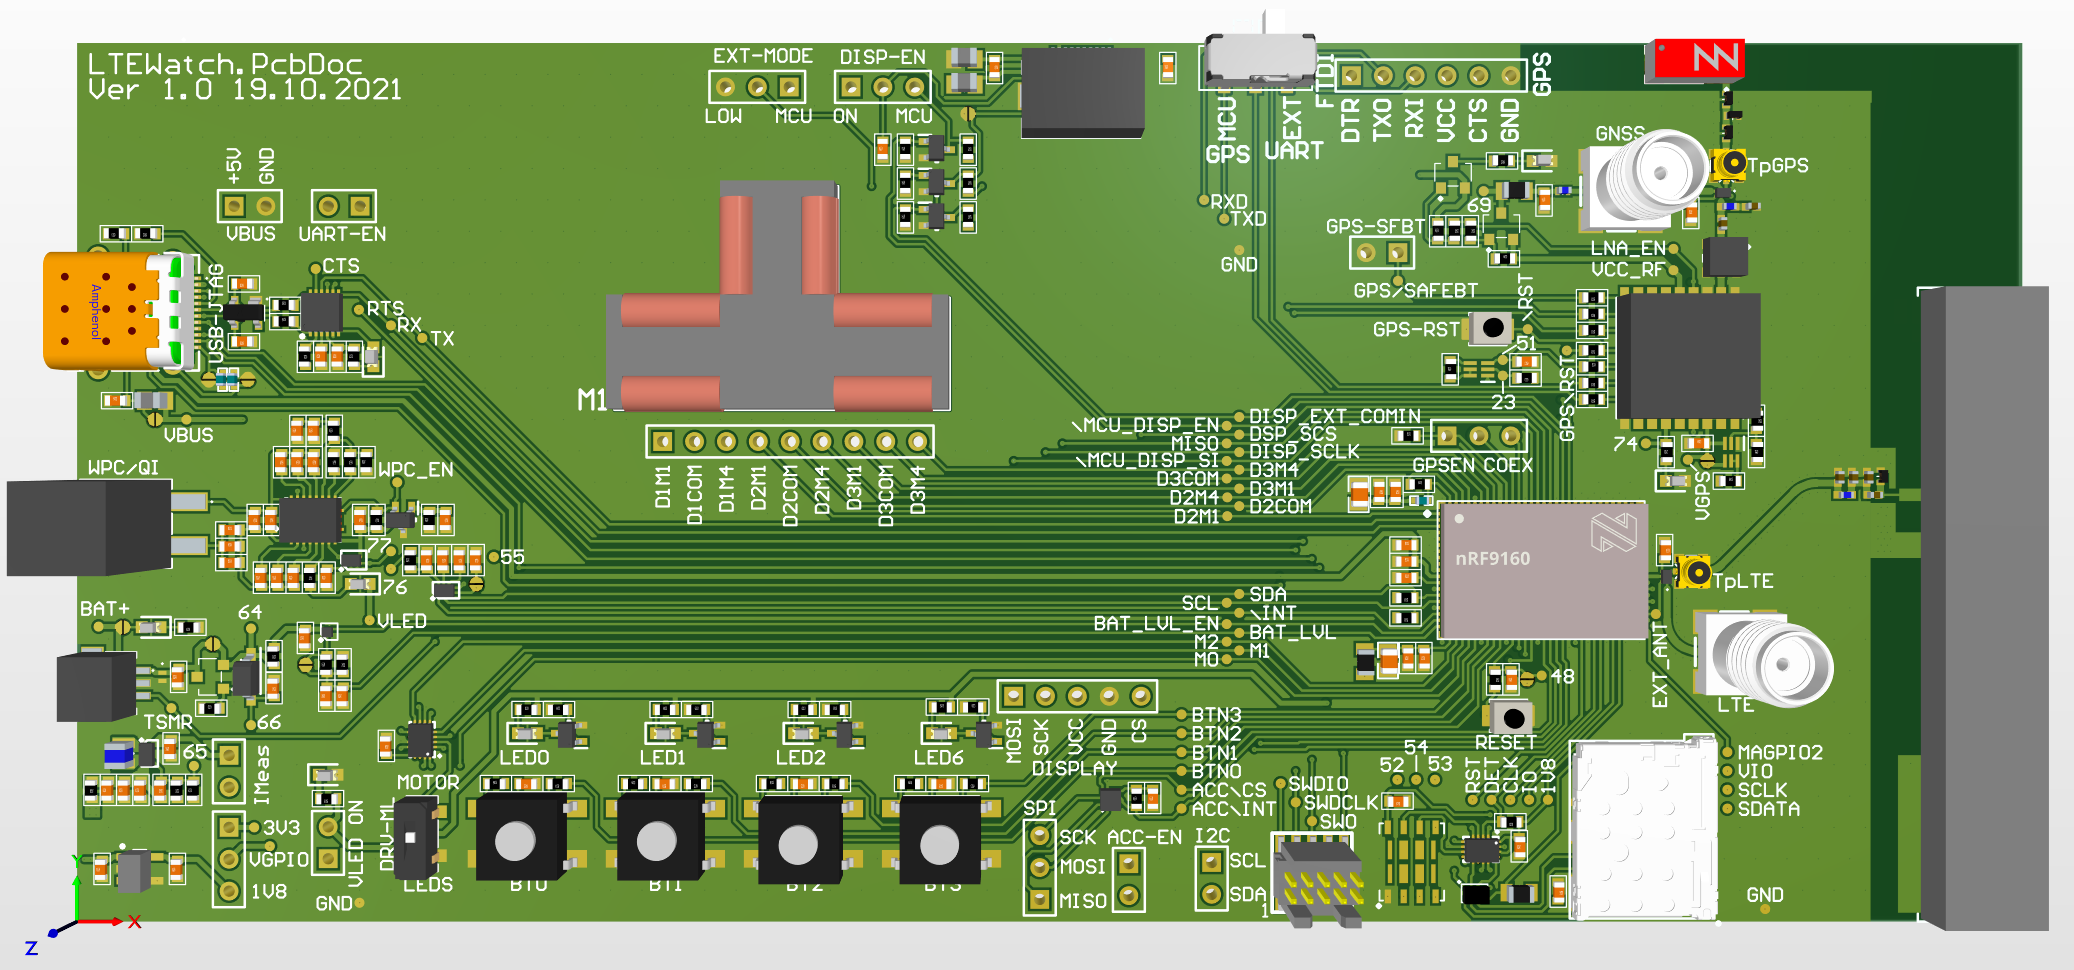
\includegraphics[width=1\textwidth]{Include/Figure/Hardware/pcb_board.png}
	\caption{Prototype PCB of the \textit{LTEWatch}}
	\label{fig:pcb_board}
\end{figure}

Due to time constraints, it was agreed with the project manager \textsc{Rieder Medard}, to let the \textit{PCB} rooting task to Steve Gallay from the HEVS (HES-SO Valais).\\

The \textit{LTEWatch} prototype board illustrated in figure \ref{fig:pcb_board} is similar to the one shown in figure \ref{fig:board_struct}. 

\begin{figure}[H]
	\centering
	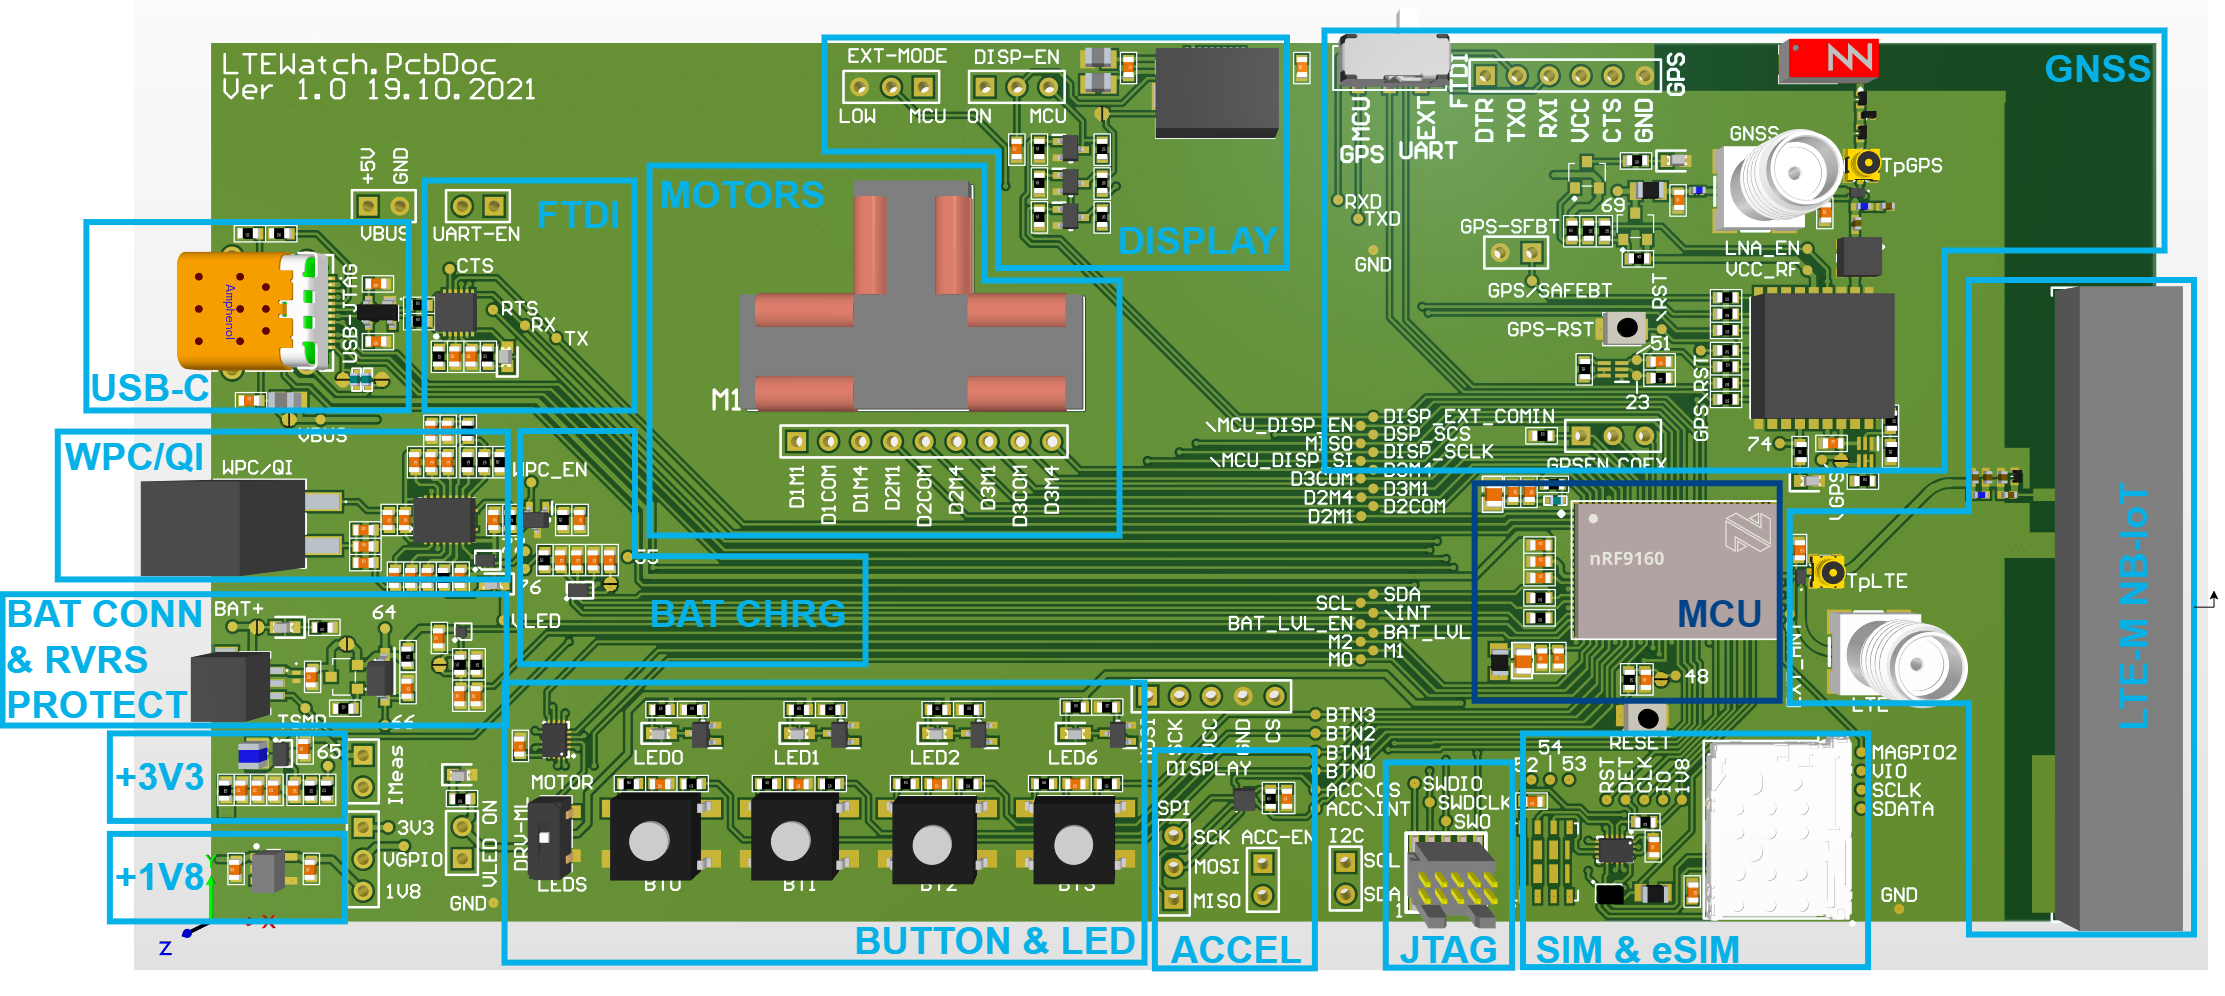
\includegraphics[width=1\textwidth]{Include/Figure/Hardware/pcb.png}
	\caption{Prototype PCB of the \textit{LTEWatch} With Annotations}
	\label{fig:pcb}
\end{figure}

\end{document}
